\documentclass[12pt]{book}
\usepackage{paralist}
\usepackage{classlog} % see geometry.pdf on how to lay out the page. There's lots.
%\usepackage{geometry} % see geometry.pdf on how to lay out the page. There's lots.
\usepackage[left=2cm, right=2cm, top=2cm]{geometry}
\geometry{a4paper} % or letter or a5paper or ... etc
\usepackage{graphicx}
% \geometry{landscape} % rotated page geometry
% See the ``Article customise'' template for come common customisations
\usepackage{amssymb}
\usepackage{amsmath}
\usepackage{imakeidx}
\usepackage[italian]{babel}
\usepackage{fancyvrb}
\usepackage[table]{xcolor}
\usepackage{tikz}
\usepackage{labinbook}
\usepackage{multirow}
\usepackage{wrapfig}
\usepackage[final]{pdfpages}
%\usepackage{nomencl}
%\makenomenclature
%\usepackage{polimiexam}
%\usepackage{lgrind}
\usetikzlibrary{arrows,shapes,backgrounds}

\makeindex

\title{\huge{\textbf{Fondamenti di Informatica} $\diamond$ \huge{\textbf{2019-20}}} \ \\ \ \\ \Large{\textbf{Lezioni, Esercitazioni e Laboratorio}}
\author{Cristiana Bolchini}}
\date{} % delete this line to display the current date


\usepackage{framed}
\usepackage{enumerate}

\renewenvironment{shaded}{%
  \def\FrameCommand{\fboxsep=\FrameSep \colorbox{shadecolor}}%
  \MakeFramed{\advance\hsize-\width \FrameRestore\FrameRestore}}%
 {\endMakeFramed}

\newenvironment{tags}[1][198,226,255]{
  \definecolor{shadecolor}{RGB}{#1}%
  \begin{snugshade}%
%  {\small 
  {\small \noindent\textbf{Argomenti:}}
}{%
%  }
    \end{snugshade}%
}

\newenvironment{esame}[1][240,244,193]{
  \definecolor{shadecolor}{RGB}{#1}%
  \begin{snugshade}%
%  {\small 
  {\small \noindent\textit{Tratto dal tema d'esame del}}
}{%
%  }
    \end{snugshade}%
}

\newcommand*{\mysep}[1]{%
 \noindent\rule{\textwidth}{1pt}%
}

\newcommand*{\prosep}[1]{%
 \noindent\rule{\textwidth}{0.75pt}%
}

\DefineVerbatimEnvironment{coding}{Verbatim}%
    {showspaces,showspaces,fontsize=\footnotesize,commandchars=\\\{\}}% showspaces and showtabs only for visualizing

\pagestyle{empty}

%%% BEGIN DOCUMENT
\begin{document}
\setcounter{numex}{1}
\setcounter{numexp}{1}
\maketitle
%\begin{tikzpicture}[show background grid]
%\node[inner sep=0pt] at (0,0) {\includegraphics[width=\paperwidth,height=\paperheight]{pattern.png}};
%\end{tikzpicture}
%\vspace{60mm}
%\begin{center}
%{\huge{\textbf{Fondamenti di Informatica}} $\diamond$ {\huge{\textbf{2017-18}}}}
%
%\vspace{20mm}
%
%{\Large{\textbf{Lezioni, Esercitazioni e Laboratorio}}}
%
%\vspace{10mm}
%
%{\Large{Cristiana Bolchini}}
%\end{center}

%\nomenclature{\texttt{while}}{costrutto ciclico a condizione iniziale}
%\nomenclature{\texttt{do-while}}{costrutto ciclico a condizione finale}
%\nomenclature{\texttt{for}}{costrutto ciclico a conteggio, a condizione iniziale}



\pagenumbering{Roman} 
\sectionbreak

\tableofcontents


\sectionbreak
\pagenumbering{arabic} 
\pagestyle{main}



%\newcommand{\nex}{\theex~\refstepcounter{ex}}
\foo{Z}{introduzione al corso}{16-09-2019}{}
%\input{2017-09-16}

\foo{Z}{la rappresentazione dell'informazione -- parte 1}{17-09-2019}{}
%\begin{itemize}
  \item  i numeri naturali
  \begin{itemize}
     \item conversione di base: 
     \begin{itemize}
    	\item dalla base 10 alla base 2
    	\item dalla base 2 alla base 10
    	\item dalla base 2 alla base 16
    	\item dalla base 16 alla base 2
    \end{itemize}
    \item aritmetica in base 2: 
    \begin{itemize}
    	\item somma
    	\item sottrazione
	   \item overflow
    \end{itemize}
  \end{itemize}
\item  i numeri relativi 
  \begin{itemize}
     \item notazione in modulo e segno
     \begin{itemize}
    		\item rappresentazione
    		\item aritmetica
	  \end{itemize}	
     \item notazione in complemento a 2
     \begin{itemize}
    		\item rappresentazione
    		\item aritmetica
	  \end{itemize}	
  \end{itemize}
\end{itemize}
\mysep{}



\foo{Z}{la rappresentazione dell'informazione -- parte 2}{19-09-2019}{}
%\input{2019-09-19}
%
\foo{Z}{algoritmi}{23-09-2019}{}
dal problema all'algoritmo 

\begin{itemize}
\item  propriet\`a dell'algoritmo
    \begin{itemize}
    \item non ambiguo
    \item deterministico
    \item termina in un numero finito di passi
   	\end{itemize}	
\item  tipologia di istruzioni
    \begin{itemize}
    \item istruzioni effettive
    \item istruzioni di controllo
    \end{itemize}   
\end{itemize}

diagrammi di flusso

\begin{itemize}
\item  blocchi elementari
    \begin{itemize}
    \item inizio
    \item fine
    \item istruzioni semplici
    \item visualizzazione risultati
    \item blocco di selezione
    \end{itemize}   
\end{itemize}

\mysep{}

\subsection{Tempo espresso in ore, minuti e secondi}
Si realizzi l'algoritmo che acquisito un valore intero (senz'altro positivo) che rappresenta una quantit\`a di tempo espressa in secondi, di calcola e visualizza la stessa quantit\`a di tempo espressa in ore, minuti e secondi. Per esempio, se si inserisce 3812, l'algoritmo calcola e visualizza 1 (ora) 3 (minuti) 32 (sec).

\begin{center}
    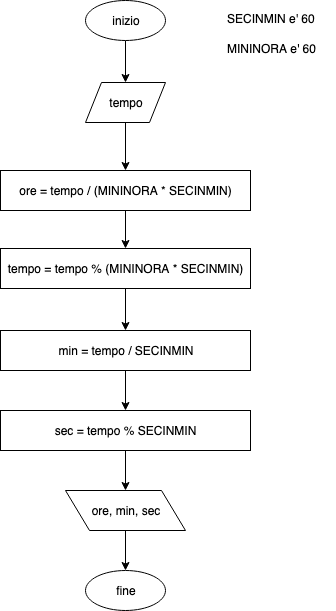
\includegraphics[width=0.3\textwidth]{./tempo.png}
\end{center}


\subsection{Operazioni di somma e sottrazione in modulo e segno}
Si realizzi l'algoritmo che acquisito un operatore (\texttt{'+'} o \texttt{'-'}) e due operandi effettua l'operazione e visualizza il risultato.

\begin{center}
    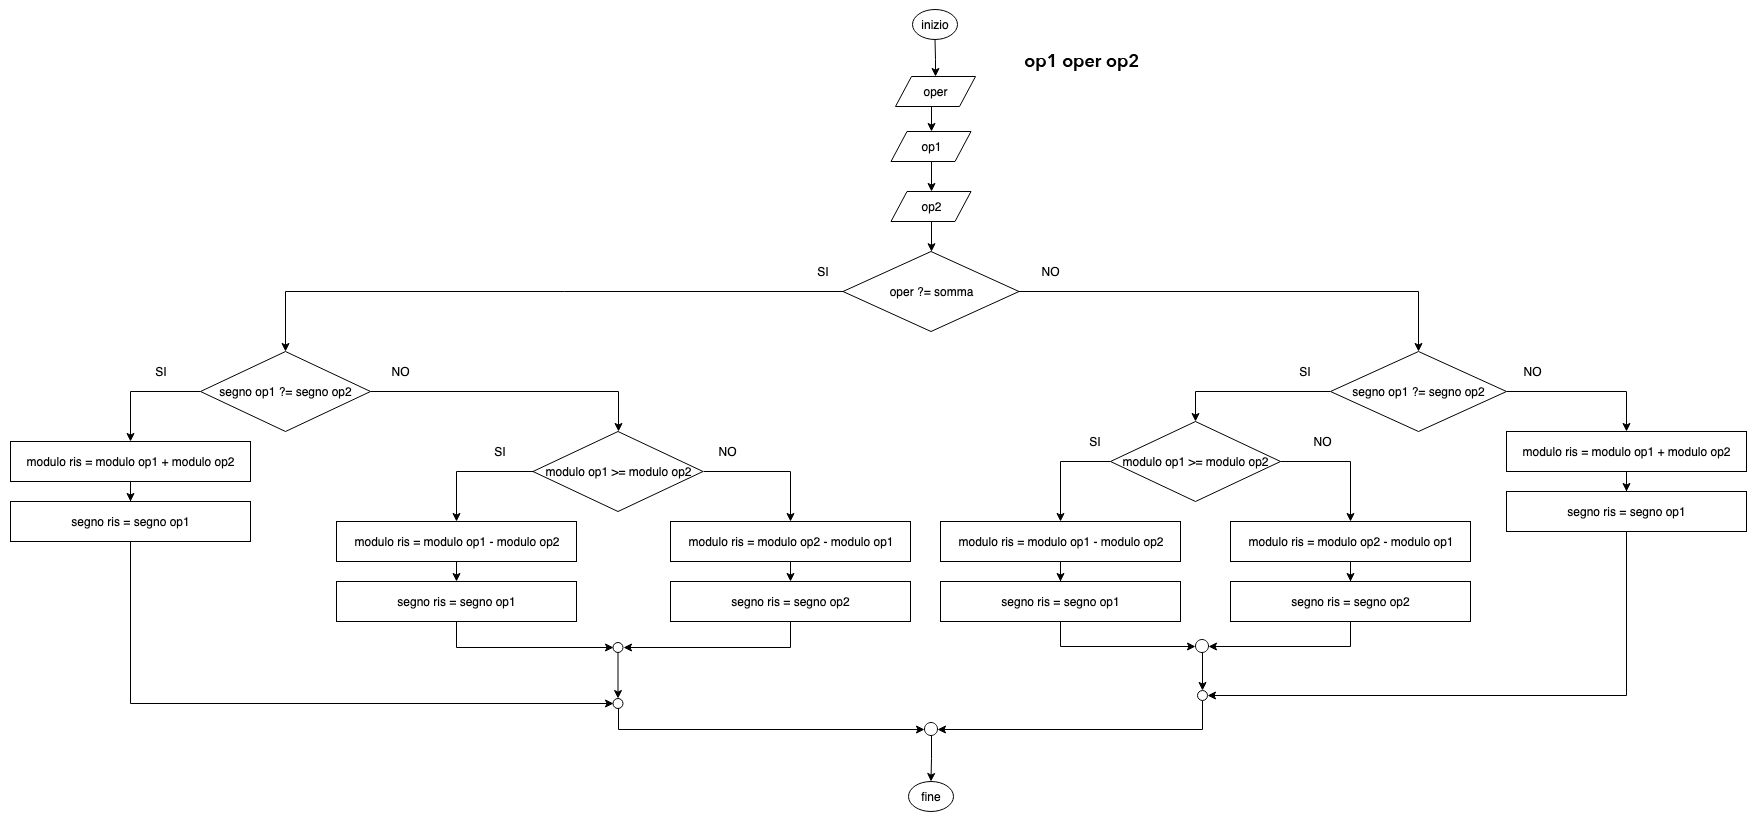
\includegraphics[width=0.9\textwidth]{./sommamodulosegno.png}
\end{center}


\subsection{Valore assoluto}
Si realizzi l'algoritmo che acquisito un valore intero calcola e visualizza il suo valore assoluto.

\begin{center}
    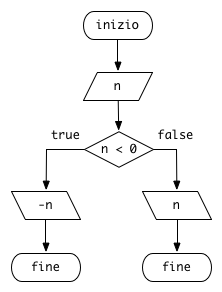
\includegraphics[width=0.3\textwidth]{./abs-alg1.png}
\end{center}

In questo caso l'algoritmo non calcola il valore assoluto, ma lo visualizza direttamente. Guardando la soluzione come una scatola nera, si ottiene il risultato richiesto, quindi soddisfa il comportamento atteso. Non rispetta la richiesta di calcolare il valore e poi visualizzarlo, ma questo aspetto \`e invisibile esternamente.
Ci sono pi\`u \texttt{fine}, aspetto poco pulito perch\'e diventa difficile riconciliare l'algoritmo.

\begin{center}
    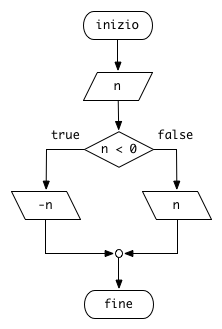
\includegraphics[width=0.3\textwidth]{./abs-alg2.png}
\end{center}

Anche in questo caso non si calcola il valore assoluto, ma si visualizza il risultato. \`E pi\`u pulito l'utilizzo di un unico punto di \texttt{fine}.

\begin{center}
    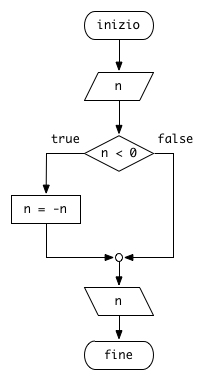
\includegraphics[width=0.3\textwidth]{./abs-alg3.png}
\end{center}

Questo algoritmo effettivamente calcola il valore assoluto e poi lo visualizza. Di fatto sovrascrive il valore iniziale con il valore assoluto, quindi eventualmente si perde questa informazione. Dal punto di vista della scatola nera, anche questa soluzione fa ci\`o che \`e richiesto.

\begin{center}
    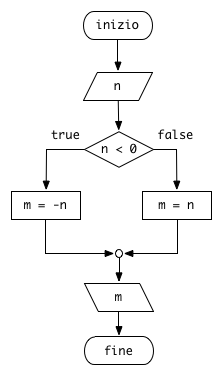
\includegraphics[width=0.3\textwidth]{./abs-alg4.png}
\end{center}

Questo algoritmo ha il comportamento richiesto e non perde il dato iniziale. L'approccio \`e migliore non tanto in relazione allo specifico problema (estremamente semplice) ma in termini di ``buone'' soluzioni, considerando che\begin{itemize} 
\item pu\`o essere necessario non tanto visualizzare il valore assoluto, ma utilizzarlo per ulteriori computazioni
\item il ``costo'' di un elemento in pi\`u per memorizzare il valore assoluto \`e irrisorio.
\end{itemize}


\foo{Z}{introduzione al C: struttura, tipi, operatori}{24-09-2019}{}
\begin{itemize}
\item struttura di un programma
    \begin{itemize}
    \item dichiarazione di variabili
    \item elaborazione
    \item visualizzazione dei risultati
    \end{itemize}
\item istruzioni
\item commenti \texttt{/* */}
\item tipi di dati di base: \texttt{int}, \texttt{float}, \texttt{double}, \texttt{char}
\item \texttt{return 0}
\item \texttt{\#define}
\item input / output formattato
    \begin{itemize}
    \item acquisizione formattata \texttt{scanf}
    \item visualizzazione \texttt{printf}
    \end{itemize}
\end{itemize}

\mysep{}


\subsection{Tempo in ore, minuti e secondi}\stepcounter{numex}
Scrivere un programma che acquisito un valore intero che rappresenta un lasso di tempo espresso in secondi calcola e visualizza lo stesso tempo in ore, minuti e secondi.

\begin{tags}
assegnamento. commenti \texttt{/* */}, operatori.
\end{tags}


\lstinputlisting[language=c]{srccode/tempoinsec.c}

Versione alternativa. Il numero di operazioni eseguite \`e lo stesso e le variabili risparmiate non fanno la differenza.

\lstinputlisting[language=c]{srccode/tempoinsec.v2.c}


\foo{Z}{costrutto di selezione \texttt{if}, \texttt{if-else}, \texttt{if-else-if}}{26-09-2019}{}
\begin{itemize}
\item cast implicito ed esplicito
\item costrutto di selezione \texttt{if}, \texttt{if-else}, \texttt{if-else-if}\index{Costrutti!\texttt{if}}\index{Costrutti!\texttt{if-else}}\index{Costrutti!\texttt{if-else if}}
    \begin{itemize}
    \item valutazione dell'espressione tra parentesi
    \item \texttt{if (a)} equivale a \texttt{if(a != 0)} e \texttt{if(!a)} equivale \texttt{if(0 == a)} 
    \item attenzione al \texttt{==} (meglio scrivere \texttt{if(\_costante\_ == \_variabile\_)})
    \item semantica di \texttt{if(a = b)}
    \item ordine di valutazione delle condizioni composte
    \item relazione tra \texttt{else} e \texttt{if} in assenza di parentesi
    \end{itemize}
\item De Morgan
\end{itemize}

\mysep{}

\subsection{Positivo, negativo o nullo}\stepcounter{numex}
Scrivere un programma che acquisito un valore visualizza \texttt{+} se positivo, \texttt{-} se negativo, \texttt{\ } altrimenti, seguito da un carattere a-capo \texttt{'\textbackslash n'}.

\begin{tags}
costrutto \texttt{if}
\end{tags}

\getsol{srccode/posnegnul.c}

Versione alternativa.

\getsol{srccode/posnegnul.v2.c}

Versione con \texttt{\#define}.

\getsol{srccode/posnegnul.v3.c}

\subsection{Anno bisestile}\stepcounter{numex}
Scrivere un programma che acquisito un valore intero positivo che rappresenta un anno, visualizza 1 se l'anno \`e bisestile\index{Programmi!Anno bisestile}, 0 altrimenti.

\begin{tags}
algoritmo. divisore/multiplo\index{divisore/multiplo}.
\end{tags}

\getsol{srccode/bisestile.c}

\prosep{}

\subsection{Terna pitagorica\index{Programmi!Terna pitagorica} -- Proposto}\stepcounter{numexp}
Scrivere un programma che acquisiti tre valori interi visualizzi 1 se costituiscono una terna pitagorica, 0 altrimenti.

\subsection{Ordinamento crescente/decrescente -- Proposto}\stepcounter{numexp}
Scrivere un programma che acquisisca un carattere e tre valori interi. Se il carattere \`e \texttt{+} visualizza i tre valori in ordine crescente, se \`e \texttt{-} li visualizza in ordine decrescente.

\begin{tags}
costrutto \texttt{if}\index{if@\texttt{if}}. algoritmo.
\end{tags}

\getsol{srccode/num3ordinatiupdown.c}

%
\foo{L}{introduzione all'ambiente di lavoro}{26-09-2019}{}
\begin{labex}{Conversione del tempo in ore, minuti e secondi}\stepcounter{numex}
Scrivere un programma che acquisito un valore intero positivo che rappresenta una durata temporale espressa in secondi, calcoli e visualizzi lo stesso intervallo di tempo espresso in ore, minuti e secondi.

\begin{tags}
algoritmo
\end{tags}

\begin{labexinout}
\labexin{un numero intero}
\labexout{tre interi separati da uno spazio (seguito da un carattere \texttt{'a-capo'})}
\end{labexinout}

\begin{labexcases}
\labexcin{453}
\labexcout{0 7 33}

\labexcin{43268}
\labexcout{12 1 8}

\end{labexcases}


\getsol{srccode/tempoinsec.c}

\end{labex}


\begin{labex}{Resto}\stepcounter{numex}
Scrivere un programma che acquisisce un intero e calcola e visualizza il numero di monete da 2 euro, 1 euro, 50, 20, 10, 5, 2 e 1 centesimo.

\begin{tags}
algoritmo
\end{tags}

\begin{labexinout}
\labexin{un numero intero}
\labexout{otto numeri interi}
\end{labexinout}

\begin{labexcases}
\labexcin{453}
\labexcout{2 0 1 0 0 0 1 1}

\labexcin{188}
\labexcout{0 1 1 1 1 1 1 1}

\end{labexcases}


\getsol{srccode/resto.c}

\end{labex}


\foo{Z}{costrutto cicliclo \texttt{while} e \texttt{do-while}}{30-09-2019}{}
\begin{itemize}
\item costrutto ciclico \texttt{while}\index{Costrutti!\texttt{while}}
    \begin{itemize}
    \item valutazione dell'espressione tra parentesi
    \item esecuzione del corpo solo se l'espressione \`e vera
    \item l'istruzione che aggiorna l'espressione  \`e tipicamente l'ultima del corpo del ciclo
    \end{itemize}
\item costrutto ciclico \texttt{do-while}\index{Costrutti!\texttt{do-while}}
    \begin{itemize}
    \item valutazione dell'espressione tra parentesi
    \item esecuzione del corpo almeno una volta 
    \end{itemize}
\end{itemize}

\mysep{}

\subsection{Minimo, massimo e valor medio}\stepcounter{numex}
Scrivere un programma che acquisisce una sequenza di 53 valori interi e calcola e visualizza valor minimo, valor massimo e media dei valori.\\index{Programmi!Minimo, massimo e valor medio} 

\begin{tags}
costrutto \texttt{while}\index{while@\texttt{while}}
\end{tags}

\lstinputlisting[language=c]{srccode/minmaxmed53.c}

\subsection{Fattoriale}\stepcounter{numex}
Chiedere all'utente un valore non negativo, e fino a quando non \`e tale ripetere la richiesta, quindi calcolare e visualizzare il fattoriale\index{Programmi!Fattoriale}.

\begin{tags}
costrutto \texttt{while}\index{while@\texttt{while}}, costrutto \texttt{do-while}\index{do-while@\texttt{do-while}}.
\end{tags}

\lstinputlisting[language=c]{srccode/fattoriale.c}

versione alternativa che distingue il caso limite $num=0$ e $num=1$ inutilmente.

\lstinputlisting[language=c]{srccode/fattorialeno.c}

versione alternativa che distrugge inutilmente il valore iniziale senza un reale risparmio

\lstinputlisting[language=c]{srccode/fattorialeno2.c}


%

\foo{E}{costrutti elementari di controllo}{01-10-2019}{}
\subsection{Conversione in binario, allo specchio}\stepcounter{numex}
Scrivere un programma che acquisito un valore intero positivo visualizza la sua rappresentazione in base 2 (con i bit in ordine inverso).

\begin{tags}
algoritmo. resto della divisione, \texttt{\#define}\index{define@\texttt{\#define}}.
\end{tags}

\lstinputlisting[language=c]{srccode/dec2bin.rev.c}

\subsection{Potenza del 2}\stepcounter{numex}
Scrivere un programma che acquisito un valore \texttt{n} intero positivo calcola e stampa la prima potenza del 2 superiore ad \texttt{n}.

\begin{tags}
algoritmo. cicli, \texttt{while}\index{while@\texttt{while}}, \texttt{\#define}\index{define@\texttt{\#define}}.
\end{tags}

\lstinputlisting[language=c]{srccode/minpow2.c}

\subsection{Numero di cifre di un valore}\stepcounter{numex}
Scrivere un programma che acquisito un valore intero calcola e visualizza il numero di cifre di cui \`e composto.

\lstinputlisting[language=c]{srccode/sizenum.c}

\subsection{Einstein}\stepcounter{numex}
Si dice che Einstein si divertisse molto a stupire gli amici con il gioco qui riportato.

Scrivete il numero 1089 su un pezzo di carta, piegatelo e datelo ad un amico che lo metta da parte. Ci\`o che avete scritto non deve essere letto fino a che non termina il gioco.

A questo punto chiedere ad una persona di scrivere 3 cifre qualsiasi (ABC), specificando che la prima e l'ultima cifra devono differire di almeno due ($|A-C| >=2$). Per fare atmosfera, giratevi e chiudete gli occhi. Una volta scritto il numero di tre cifre, chiedete all'amico di scrivere il numero che si ottiene invertendo l'ordine delle cifre (CBA). A questo punto fate sottrarre dal numero pi\`u grande quello pi\`u piccolo: $XYZ = |ABC - CBA|$ e fate anche calcolare il numero che si ottiene invertendo le cifre del numero risultante: ZYX. Infine, fate sommare questi ultimi due numeri: XYZ + ZYX e constatate che il risultato \`e 1089.

Fate estrarre il foglio tenuto da parte fino a questo momento: 1089!

Realizzate un programma che fa i seguenti passi:\begin{itemize}
\item    Chiede all'utente di inserire un numero di 3 cifre, specificando il vincolo tra la prima e l'ultima cifra, e se i vincoli non sono rispettati chiede nuovamente il valore
\item    Acquisisce il valore
\item    Visualizza il numero inserito e il numero con le cifre in ordine inverso
\item    Visualizza la differenza tra i due valori (deve essere un numero positivo)
\item    Visualizza il numero con le cifre in ordine inverso
\item    Visualizza il risultato della somma tra questi due valori (dovrebbe essere 1089 per qualsiasi numero di 3 cifre che rispetta il vincolo tra la prima e l'ultima cifra)
\end{itemize}

\lstinputlisting[language=c]{srccode/einstein.c}

\prosep{}

\subsection{Conversione in binario, senza array -- Proposto e risolto}\stepcounter{numex}
Acquisire un valore intero e calcolare e visualizzare la sua rappresentazione nel sistema binario, mostrando le cifre nell'ordine corretto. Se l'utente inserisce 6, il valore visualizzato \`e 110.
Il suggerimento \`e che un numero binario pu\`o anche essere visto come un numero in base dieci, ossia 110 in binario pu\`o anche essere visto come centodieci in decimale ...

\begin{tags}
algoritmo. resto della divisione, \texttt{\#define}\index{define@\texttt{\#define}}. moltiplicazioni ripetute per la base.
\end{tags}

\lstinputlisting[language=c]{srccode/dec2bin.noarray.c}

\subsection{Conversione in binario, allo specchio, con dimensione}\stepcounter{numexp}
Scrivere un programma che acquisisce un primo valore intero, il dato da convertire in binario, ed un secondo dato intero, il numero di bit su cui rappresentarlo. Il programma visualizza la rappresentazione in base 2 (con i bit in ordine inverso) del valore acquisito, eventualmente aggiungendo bit di padding.

\lstinputlisting[language=c]{srccode/dec2bin.dimrev.c}


\foo{X}{lauree}{03-10-2019}{}
%\input{2019-10-03.if}

%
\foo{Z}{array monodimensionali e ciclo \texttt{for}}{07-10-2019}{}
\begin{itemize}
\item array monodimensionali
\item dati di tipo omogeneo
\item dimensione dell'array costante e nota a priori
\item indice degli elementi da \texttt{0} a \texttt{dimensione} - 1
\item costrutto ciclico a conteggio \texttt{for} (a condizione iniziale)
\item le tre parti del costrutto
\begin{itemize}
	\item istruzioni prima di iniziare il ciclo
	\item condizioni, semplici e composte
	\item istruzioni a chiusura del corpo del ciclo
  \end{itemize}
\item separatore per le istruzioni nella prima e terza parte del costrutto
\item parti sono facoltative
\end{itemize}

\mysep{}


\subsection{5 dati in ingresso in ordine inverso}\stepcounter{numex}
Scrivere un programma che acquisiti 5 numeri interi li visualizza in ordine inverso.

\begin{tags}
array monodimensionale. cicli a conteggio. costrutto \texttt{for}\index{for@\texttt{for}}.
\end{tags}

\lstinputlisting[language=c]{srccode/rev5noarray.c}

Versione con array.

\lstinputlisting[language=c]{srccode/rev5.c}


\subsection{Sopra soglia}\stepcounter{numex}
Scrivere un programma che acquisisce 20 valori interi, quindi un intero valore soglia e calcola e visualizza in numero di campioni strettamente superiori alla soglia.

\lstinputlisting[language=c]{srccode/soprasoglia.c}

Versione con il costrutto \texttt{for}.

\lstinputlisting[language=c]{srccode/soprasoglia-for.c}

\prosep{}

\subsection{Conversione in binario -- Proposto}\stepcounter{numexp}
Scrivere un programma che acquisisce un valore compreso tra 0 e 1023, estremi inclusi e finch\'e non \`e tale lo richiede. Quindi effettua la conversione in base 2 e la visualizza.

\begin{tags}
algoritmo. validazione ingresso. dimensione dell'array.
\end{tags}

\lstinputlisting[language=c]{srccode/dec2bin.c}

Versione alternativa con ciclo \texttt{do-while}.

\lstinputlisting[language=c]{srccode/dec2bin2.c}

Versione alternativa in cui si visualizza il numero sul numero completo di bit massimo.

\lstinputlisting[language=c]{srccode/dec2binallbits.c}




%
\foo{E}{array monodimensionali}{08-10-2019}{}
\subsection{Numero allo specchio}\stepcounter{numex}
Scrivere un programma in C che acquisito un valore intero calcola e visualizza il valore ottenuto invertendo l'ordine delle cifre che lo compongono. Ad esempio, se il programma acquisisce il valore 251, il programma visualizza 152. Si ipotizzi (non si devono far verifiche in merito) che il valore acquisito non dia problemi di overflow e sia senz'altro strettamente positivo. Se l'utente inserisce il valore 1000, il programma visualizza 1 (questo perch\`e CALCOLA e poi visualizza). Se l'utente inserisce 9001 il programma visualizza 1009.

\begin{tags}
algoritmo.
\end{tags}

\begin{esame}
04/09/2015 (Variante)
\end{esame}
   
\lstinputlisting[language=c]{srccode/mirrornum.c}


\subsection{Conta lettere}\stepcounter{numex}
Scrivere un programma\index{Programmi!Conta occorrenze caratteri} che acquisisce una sequenza di 50 caratteri e per ogni carattere letto mostra quante volte compare nella sequenza, mostrandoli in ordine alfabetico. Si consideri che i caratteri inseriti siano tutti caratteri minuscoli.
Per esempio, se l'utente inserisce \texttt{sequenzadiprova} (solo 16 caratteri in questo caso, per questioni di leggibilit\`a), il programma visualizza
\begin{verbatim}
a 2
d 1
e 2
i 1
n 1
o 1
p 1
q 1
r 1
s 1
u 1
v 1
z 1
\end{verbatim}

\begin{tags}
array monodimensionale. cicli a conteggio. contatori di occorrenze. codice ASCII di un carattere. costrutto \texttt{for}\index{for@\texttt{for}}.
\end{tags}

\lstinputlisting[language=c]{srccode/contacarinseq.c}

\subsection{Niente primi}\stepcounter{numex}
Scrivere un programma che acquisisce una sequenza di al pi\`u 50 valori interi strettamente maggiori di 1 e che si ritiene terminata quando l'utente inserisce un valore minore o uguale a 1. Il programma, una volta acquisiti i dati, visualizza 1 se tra di essi non c'\`e alcun numero primo\index{Programmi!Numero primo}, 0 altrimenti.

\begin{tags}
array monodimensionale. cicli annidati. numero primo.
\end{tags}

\lstinputlisting[language=c]{srccode/noprime.c}

%
\foo{Z}{array bidimensionali, \texttt{struct} e \texttt{typedef}}{10-10-2019}{}
\begin{itemize}
\item array pluri-dimensionali: dimensione 2
\begin{itemize}
\item scansione mediante due cicli annidati
\item linearizzazione della memoria
\end{itemize}
\item \texttt{struct}   
	\begin{itemize}
	\item nome facoltativo, ma sempre utilizzato
	\item array di \texttt{struct}
	\item \texttt{struct} con campo array
    \end{itemize}
\item \texttt{typedef}
\end{itemize}

\mysep{}

%\subsection{Palindrome}
%Scrivere un programma che acquisita una sequenza di 15 caratteri visualizza 1 se si tratta di un vocabolo palindrome\index{Programmi!Palindrome}, 0 altrimenti.
%
%\begin{tags}
%algoritmo. variabile di controllo che rappresenta il risultato.
%\end{tags}
%
%
%\getsol{srccode/palindrome.c}

\subsection{Matrice identit\`a}\stepcounter{numex}
Si scriva un programma che acquisisce i dati di una matrice di dimensione \texttt{5x5} di valori interi. Il programma visualizza 1 se si tratta di una matrice identit\`a, 0 altrimenti.

\begin{tags}
array bidimensionali. algoritmo.\index{Programmi!Matrice identit\`a}
\end{tags}

\getsol{srccode/matidentita.c}

\noindent\makebox[\linewidth]{\rule{\textwidth}{0.6pt}}

\subsection{Date: definizione di tipo}\stepcounter{numex}
Definire un nuovo tipo di dato, cui dare nome \texttt{date\_t} , per rappresentare date in termini di giorno, mese ed anno.
\begin{tags}
\texttt{typedef}\index{typedef@\texttt{typedef}}.
\end{tags}

\begin{lstlisting}[language=c]
typedef struct date_s {
   int g, m, a;
} date_t;
\end{lstlisting}

\subsection{Studente: definizione di tipo}\stepcounter{numex}
Definire un nuovo tipo di dato, cui dare nome \texttt{student\_t} per rappresentare le informazioni seguenti relative ad uno studente:
\begin{itemize}
\item cognome e nome: due array di caratteri di 41 caratteri ciascuno
\item data di nascita e data di immatricolazione: due data
\item voti esami: un array di NESAMI interi (dovete saperlo voi)
\item media: voto medio (relativo agli esami superati)
\item livello: 'T' o 'M' per distinguere se si \`e immatricolati alla triennale o alla magistrale. 
\end{itemize}

\begin{tags}
\texttt{typedef}\index{typedef@\texttt{typedef}}.
\end{tags}

\begin{lstlisting}[language=c]
#define NL 41
#define NESAMI 18
typedef struct student_s {
   char last[NL+1], first[NL]+1;
   date_t dnascita, dlaurea;
   int grades[NEX];
   float avg;
   char level;
} student_t;
\end{lstlisting}




\foo{Z}{stringhe}{14-10-2019}{}
\begin{itemize}
\item sequenza di caratteri delimitata dal terminatore '\texttt{\textbackslash 0}'
\item allocazione dell'array con \texttt{N+1} elementi
\item acquisizione    \begin{itemize}
	\item \texttt{scanf}: segnaposto \texttt{\%s} e niente \texttt{\&} davanti al nome dell'array
	\item \texttt{gets}: serve poi solo il nome dell'array, trattandosi \textit{sempre} di caratteri
    \end{itemize}
\item scansione con condizione \texttt{s[i] != '\textbackslash 0'}
\end{itemize}
\mysep{}

\subsection{Stringa allo specchio}\stepcounter{numex}
Scrivere un programma che acquisisce una stringa di al pi\`u 25 caratteri, inverte l'ordine di tutti i caratteri in essa contenuta e la visualizza.

\begin{tags}
stringa. algoritmo.
\end{tags}

\getsol{srccode/stringaallospecchio.c}

\subsection{Stringa allo specchio senza vocali}\stepcounter{numex}
Scrivere un programma che acquisisce una stringa di al pi\`u 25 caratteri, inverte l'ordine di tutti i caratteri ed elimina tutte le vocali in essa contenute. Ci sono solo caratteri minuscoli.

\begin{tags}
stringa. algoritmo.\index{Programmi!Inverti stringa}
\end{tags}

\getsol{srccode/mirrornovoc.c}

versione alternativa

\getsol{srccode/mirrornovoc2.c}

\subsection{Anagrammi}\stepcounter{numex}
Scrivere un programma che acquisisce due stringhe di al pi\`u 20 caratteri e determina se una sia l'anagramma\index{Programmi!Anagramma} dell'altra, visualizzando 1 in caso affermativo, 0 altrimenti.
\begin{tags}
algoritmo. stringhe. dimensione dell'array.
\end{tags}

\getsol{srccode/anagramma.c}

\foo{F}{array}{15-10-2019}{}
\begin{exrev}{Numeri vicini}\stepcounter{numex}
Scrivere un programma in C che chiede all'utente di inserire una sequenza di numeri interi terminata dallo 0 (lo 0 non fa parte della sequenza). Il programma ignora i valori negativi e valuta e stampa a video le coppie di numeri consecutivi che soddisfano tutte le condizioni che seguono:\begin{itemize}
\item sono diversi tra di loro,
\item sono entrambi numeri pari,
\item il loro prodotto \`e un quadrato perfetto.
\end{itemize}


\begin{tags}
algoritmo. numeri pari. quadrato perfetto
\end{tags}

\lstinputlisting[language=c]{srccode/adiacentivincolati.c}

\end{exrev}

\begin{exrev}{Distanza di Hamming}\stepcounter{numex}
Scrivere un programma che acquisiti due sequenze di 10 bit ciascuna (forniti una cifra alla volta), calcola e visualizza il vettore della distanza di Hamming, ed infine la distanza. Un esempio di esecuzione \`e il seguente:
\begin{verbatim}
1 0 0 1 0 0 1 0 0 1
1 1 1 1 0 0 0 1 0 1
0 1 1 0 0 0 1 1 0 0   4
\end{verbatim}

\begin{tags}
array monodimensionale. cicli a conteggio. costrutto \texttt{for}\index{for@\texttt{for}}.
\end{tags}

\lstinputlisting[language=c]{srccode/hamming.c}
\end{exrev}

\begin{exrev}{Carta di credito}\stepcounter{numex}
Scrivere un programma che acquisisce un numero di carta di credito Visa costituito da 13 o 16 caratteri numerici e verifica che si tratti di un numero di carta valido oppure no. Nel primo caso visualizza 1, altrimenti 0. L'algoritmo che verifica la correttezza ''sintattica`` di un numero (inventato da Hans Peter Luhn di IBM) \`e il seguente: 
\begin{wrapfigure}{r}{0.25\textwidth}
  \begin{center}%\vspace{-2em}
    \includegraphics[width=\linewidth]{srccode/cartalupin.png}
  \end{center}\vspace{-4em}
\end{wrapfigure}

\begin{itemize}
\item moltiplicare una cifra si, una no, per 2 partendo dalla penultima a destra, quindi sommare tali cifre,
\item sommare a tale valore, le cifre che non sono state moltiplicate per 2,
\item se il valore ottenuto \`e un multiplo di 10, il numero \`e valido.
\end{itemize}



Per esempio, si consideri il numero di carta di credito seguente: $4003600000000014$.
\begin{itemize}
\item moltiplicare una cifra si, una no, per 2 partendo dalla penultima a destra, quindi sommare tali cifre (sono sottolineate le cifre da moltiplicare per 2):

\underline{4}0\underline{0}3\underline{6}0\underline{0}0\underline{0}0\underline{0}0\underline{0}0\underline{1}4

si moltiplica ogni cifra per 2:

$1\times2 + 0\times2 + 0\times2 + 0\times2 + 0\times2 + 6\times2 + 0\times2 + 4\times2$

si ottiene:

$2 + 0 + 0 + 0 + 0 + 12 + 0 + 8$

si sommano le cifre:

$2 + 0 + 0 + 0 + 0 + 1 + 2 + 0 + 8 = 13$

\item sommare a tale valore, le cifre che non sono state moltiplicate per 2,

$13 + 4 + 0 + 0 + 0 + 0 + 0 + 3 + 0 = 20$

\item se il valore ottenuto \`e un multiplo di 10, il numero \`e valido: in questo caso le \`e.
\end{itemize}

Potete provare con alcuni numeri suggeriti da PayPal: 4111111111111111, 4012888888881881, 4222222111212222.

\begin{tags}
array di caratteri. corrispondenza carattere numerico valore. cicli a conteggio. cifre di un numero.
\end{tags}
\lstinputlisting[language=c]{srccode/cartadicredito.c}
\end{exrev}

\begin{exrev}{Media mobile}\stepcounter{numex}
Si scriva un programma che acquisiti 100 valori interi ed un valore intero \texttt{n} calcola e visualizza l'array di valori che costituiscono la media mobile dei dati in ingresso di finestra \texttt{n}. L'elemento \texttt{i}-esimo della media mobile viene calcolato come media degli \texttt{n} valori del vettore in ingresso che precedono e includono l'elemento \texttt{i}. Se l'elemento \texttt{i} \`e preceduto da meno di \texttt{n}-1 valori, la media si calcola su quelli.


\begin{tags}
array monodimensionali. calcolo della media.
\end{tags}

\begin{esame}
03/07/2017 (variante)
\end{esame}

\lstinputlisting[language=c]{srccode/movingavg.c}
\end{exrev}

\begin{exrev}{Conta caratteri}\stepcounter{numex}
Scrivere un programma in C che acquisisca una sequenza \texttt{str} di 20 caratteri. Per ogni carattere \texttt{car} contenuto nella stringa \texttt{str}, a partire dall'ultimo fino ad arrivare al primo, il programma visualizza (senza lasciare spazi) il carattere \texttt{car}, seguito dal numero di volte in cui compare consecutivamente in quel punto della stringa. Per esempio, se l'utente inserisce \texttt{aabbbddbbbbhhhhhzzzz} il programma visualizza \texttt{z4h5b4d2b3a2}.


\begin{tags}
array monodimensionali. caratteri. algoritmo.
\end{tags}

\begin{esame}
03/07/2017 (variante)
\end{esame}

\lstinputlisting[language=c]{srccode/contacar1.c}

\blind{Versione alternativa}

\lstinputlisting[language=c]{srccode/contacar2.c}

\blind{Versione alternativa con il costrutto \texttt{for}}

\lstinputlisting[language=c]{srccode/contacar3.c}
\end{exrev}




\foo{E}{array e stringhe}{17-10-2019}{}
\subsection{Determinante di una matrice dimensione 3}\stepcounter{numex}

Scrivere un programma che acquisisce i dati di una matrice di dimensione \texttt{3x3} di numeri interi, quindi calcola e visualizzare il determinante.
\[
A = 
\begin{bmatrix}
a_{11} & a_{12} & a_{13} \\
a_{21} & a_{22} & a_{23} \\
a_{31} & a_{32} & a_{33} \\
\end{bmatrix}
\]

{\small
$$ det(A) = a_{11}\times a_{22}  \times a_{33}  + a_{12} \times a_{23}\times a_{31}  + a_{13} \times a_{21} \times a_{32} - a_{13} \times a_{22} \times a_{31} - a_{12} \times a_{21} \times a_{33} - a_{11} \times a_{23} \times a_{32} $$}

\begin{tags}
array bidimensionale.
\end{tags}

%\lstinputlisting[language=c]{srccode/determinante3.c}

\subsection{Nome di file da percorso, nome ed estensione}\stepcounter{numex}
Scrivere un programma che acquisisce una stringa di al pi\`u 50 caratteri che contenga il nome di un file completo di percorso e visualizza il solo nome. 

\begin{tags}
stringa. algoritmo.
\end{tags}

\begin{esame}
\end{esame}

\getsol{srccode/nomefile.c}

oppure:

\getsol{srccode/nomefile2.c}


\subsection{Da intero a stringa\index{Programmi!Da intero a stringa}}\stepcounter{numex}
Scrivere un programma che acquisito un intero crea una stringa che contiene le cifre dell'intero. L'intero ha al pi\`u 6 cifre. 

\begin{tags}
stringa. algoritmo. carattere numerico.
\end{tags}

\getsol{srccode/itos.c}

Versione alternativa.

\getsol{srccode/itos2.c}

\subsection{Area di un poligono}\stepcounter{numex}
Scrivere un programma che calcola e visualizza l'area di un poligono, a partire dalle coordinate dei suoi vertici e usando la formula di Gauss.
Il poligono ha al pi\`u 10 vertici, ciascuno rappresentato dalle coordinata \texttt{x} e \texttt{y} (valori interi).
Il programma acquisisce prima il numero \texttt{num} di vertici del poligono, verificando che sia non superiore a 10, quindi acquisisce le coordinate dei \texttt{num} vertici, quindi procede al calcolo dell'area e la visualizza.
Si dichiari un opportuno tipo di dato (\texttt{vertex\_t}) per rappresentare i vertici del poligono.

\getsol{srccode/areapoligonogauss.c}


\subsection{Quadrato magico}\stepcounter{numex}
Si scriva un programma che acquisisce i dati di una matrice di dimensione \texttt{3x3} di valori interi. Il programma visualizza 1 se si tratta di un quadrato magico seguito dal valore della somma, 0 altrimenti.
Un quadrato magico \`e un insieme di numeri interi distinti in una tabella quadrata tale che la somma dei numeri presenti in ogni riga, in ogni colonna e in entrambe le diagonali dia sempre lo stesso valore.

\begin{tags}
array bidimensionali. algoritmo.
\end{tags}

\getsol{srccode/magicq1.c}

Versione alternativa.

\getsol{srccode/magicq2.c}



\foo{L}{algoritmi e array}{17-10-2019}{}
\begin{labex}{Fattori}
Scrivere un programma che acquisisce due numeri interi relativi e visualizza 1 se uno \`e un divisore dell'altro o viceversa, 0 altrimenti.
Dopo il valore visualizzato, mettere un \texttt{'a-capo'}.

\begin{labexinout}
\labexin{due numeri interi}
\labexout{un intero (seguito da un carattere \texttt{'a-capo'})}
\end{labexinout}

\begin{labexcases}
\labexcin{5542 18}
\labexcout{0}

\labexcin{5542 17}
\labexcout{1}

\labexcin{13 1950}
\labexcout{1}
\end{labexcases}

\getsol{srccode/fattori.c}

\end{labex}


\begin{labex}{Padding}
Si vuole rappresentare a video un valore naturale \texttt{num} utilizzando un numero a scelta di cifre \texttt{k} inserendo 0 nelle posizioni pi\`u significative, fino a raggiungere la dimensione desiderata. 
Per esempio, volendo rappresentare \texttt{842} su \texttt{5} cifre, si ottiene \texttt{00842}.

Scrivere un programma che acquisisce due valori interi entrambi strettamente positivi (e finch\'e non \`e cos\`i richiede il valore che non rispetta il vincolo) num e \texttt{k}, quindi rappresenta \texttt{num} su \texttt{k} cifre. Se \texttt{k} e' minore del numero di cifre presenti in \texttt{num}, il programma visualizza il valore \texttt{num} come \`e. 
Dopo il valore visualizzato, mettere un \texttt{'a-capo'}.

%\begin{tags}
%\texttt{if}\index{if@\texttt{if}}
%\end{tags}

\begin{labexinout}
\labexin{due numeri interi (da verificare)}
\labexout{un intero (seguito da un carattere \texttt{'a-capo'})}
\end{labexinout}

\begin{labexcases}
\labexcin{11304 9}
\labexcout{000011304}

\labexcin{-4 9000 -5 -2 2}
\labexcout{9000}

\labexcin{1 1}
\labexcout{1}
\end{labexcases}


\getsol{srccode/padding.c}

\end{labex}

\begin{labex}{Super Mario}

\begin{wrapfigure}{r}{0.25\textwidth}
  \begin{center}\vspace{-2em}
    \includegraphics[width=\linewidth]{srccode/pyramids-mario.png}
  \end{center}\vspace{-8em}
\end{wrapfigure}



Nella preistoria dei videogiochi in Super Mario della Nintendo, Mario deve saltare da una piramide di blocchi a quella adiacente.
Proviamo a ricreare le stesse piramidi in C, in testo, utilizzando il carattere cancelletto ($\#$) come blocco, come riportato di seguito. In realt\`a il carattere $\#$ \`e pi\`u alto che largo, quindi le piramidi saranno un po' pi\`u alte.

\begin{verbatim}
   #  #
  ##  ##
 ###  ###
####  ####
\end{verbatim}

Notate che lo spazio tra le due piramidi \`e sempre costituito da \textbf{2} spazi, indipendentemente dall'altezza delle piramidi. Inoltre, alla fine delle piramidi \textbf{non ci devono essere spazi}.
L'utente inserisce l'altezza delle piramidi, che deve essere un valore strettamente positivo e non superiore a 16. In caso l'utente inserisca un valore che non rispetta questi vincoli, la richiesta viene ripetuta.

\begin{labexinout}
\labexin{un numero intero (da verificare)}
\labexout{una sequenza di caratteri}
\end{labexinout}


\getsol{srccode/mario.c}

\end{labex}

\begin{labex}{Scorrimento a destra -- rightshift}
Scrivere un programma che acquisita una stringa di al pi\`u 10 caratteri, modifica la stringa in modo tale che la stringa finale sia quella iniziale, fatta scorrere a destra di una posizione, con l'ultimo carattere riportato in testa. Se per esempio la sequenza iniziale \`e \texttt{attraverso}, la stringa finale sar\`a \texttt{oattravers}. 
Una volta modificata la stringa memorizzata, visualizzarla e farla seguire da un carattere \texttt{'a-capo'}.

\begin{labexinout}
\labexin{al pi\`u 10 caratteri}
\labexout{al pi\`u 10 caratteri (seguiti da un carattere \texttt{'a-capo'})}
\end{labexinout}

\begin{labexcases}
\labexcin{attraverso}
\labexcout{oattravers}

\labexcin{ananas}
\labexcout{sanana}

\labexcin{trampolini}
\labexcout{itrampolin}
\end{labexcases}

\getsol{srccode/rightshift.c}

\end{labex}


\begin{labex}{Troncabile primo a destra}
Scrivere un programma che acquisisce un valore intero strettamente positivo, e finch\'e non \`e tale lo richiede. Il programma analizza il valore intero e visualizza 1 nel caso sia un troncabile primo a destra, 0 altrimenti.
Un numero si dice troncabile primo a destra se il numero stesso e tutti i numeri che si ottengono eliminando una alla volta la cifra meno significativa del numero analizzato al passo precedente, sono numeri primi.
Per esempio, se il numero iniziale \`e 719, i numeri che si ottengono ``eliminando una alla volta la cifra meno significativa del numero analizzato al passo precedente ..'' sono 71 e 7.
Dopo il valore visualizzato, mettere un \texttt{'a-capo'}.

\begin{labexinout}
\labexin{un intero (da verificare)}
\labexout{un intero (seguito da un carattere \texttt{'a-capo'})}
\end{labexinout}

\begin{labexcases}
\labexcin{719}
\labexcout{1}

\labexcin{473}
\labexcout{0}

\labexcin{-42 -18 311111}
\labexcout{0}

\labexcin{3137}
\labexcout{1}
\end{labexcases}

\getsol{srccode/troncabileprimodx.c}

\end{labex}



\foo{Z}{sottoprogrammi}{21-10-2019}{}
\begin{itemize}
\item intestazione
\item tipo di dato restituito
\item parametri formali e attuali
\item prototipo 
\item \texttt{return}
\item tipo \texttt{void}
\item passaggio array monodimensionali e dimensione
\item visibilit\`a delle variabili
\end{itemize}

\subsection{Combinazioni}\stepcounter{numex}
Scrivere un programma che acquisisce due interi \texttt{n} e \texttt{k} strettamente positivi, con \texttt{k} non superiore a  \texttt{n} e finch\`e non \`e tale li richiede (entrambi). Quindi calcola e visualizza il numero di combinazioni di \texttt{n} elementi, presi \texttt{k} per volta.

\lstinputlisting[language=c]{srccode/combinazioninosub.c}

versione con sottoprogrammi

\lstinputlisting[language=c]{srccode/combinazioni.sub.c}

\lstinputlisting[language=c]{srccode/combinazioni.c}

\subsection{Massimo di un array}\stepcounter{numex} 
Scrivere un sottoprogramma che ricevuto in ingresso un array di numeri interi e \textit{qualsiasi altro parametro ritenuto strettamente necessario} restituisce l'indice dell'elemento con valore massimo.

\begin{tags}
sottoprogrammi. passaggio array monodimensionale.
\end{tags}

\lstinputlisting[language=c]{srccode/imaxarrayint.c}


\subsection{Triangolo -- Proposto e risolto}\stepcounter{numex} 
Scrivere un sottoprogramma che ricevuti in ingresso tre interi, restituisce 1 nel caso in cui si tratti delle dimensioni dei lati di un triangolo valido 0 altrimenti. Le condizioni che devono sussistere sono:\begin{itemize}
\item le dimensioni sono positive
\item la somma di due dimensioni non \`e mai superiore alla terza dimensione
\end{itemize}

\lstinputlisting[language=c]{srccode/triangolovalido.c}



\foo{Z}{sottoprogrammi}{22-10-2019}{}
\begin{itemize}
\item passaggio parametri per copia valore, per copia indirizzo
\item record di attivazione
\end{itemize}

\subsection{Massimo, minimo e media dei valori di un array}\stepcounter{numex}
Scrivere un sottoprogramma che ricevuto in ingresso un array di numeri interi e \textit{qualsiasi altro parametro ritenuto strettamente necessario} \textit{trasmette} al chiamante l'indice dell'elemento con valore massimo, quello con valore minimo e la media dei valori dell'array.

\begin{tags}
sottoprogrammi. passaggio array monodimensionale. passaggio parametri per indirizzo.
\end{tags}

\lstinputlisting[language=c]{srccode/minmaxavgarrint.c}



\foo{E}{sottoprogrammi}{24-10-2017}{}
\begin{itemize}
\item passaggio di array bidimensionali
\item passaggio di \texttt{struct}
\end{itemize}


\subsection{Lunghezza di una stringa}\stepcounter{numex}
Scrivere il sottoprogramma che ricevuta in ingresso una stringa, calcola e
restituisce la sua lunghezza.

\getsol{srccode/mystrlen.sub.c}

\subsection{Matrice identit\`a}\stepcounter{numex}
Scrivere un sottoprogramma che ricevuto in ingresso un array bidimensionale e qualsiasi altro parametro ritenuto strettamente necessario restituisce 1 se si tratta di una matrice identit\`a, 0 altrimenti. La dimensione dell'array dichiarata \`e \texttt{N}.

\getsol{srccode/identita.sub.c}

\subsection{Vertici di un poligono}\stepcounter{numex}
Si consideri il seguente tipo di dato per rappresentare punti nello spazio piano.
\begin{lstlisting}[language=c]
typedef struct p {
    int x, y;
} punto_t;
\end{lstlisting}

Si scriva un sottoprogramma che ricevuto in ingresso un array di tipo \texttt{punto\_t} e qualsiasi altro parametro ritenuto strettamente necessario acquisisca i dati relativi ai vertici di un poligono.

\getsol{srccode/getpoints.c}

\subsection{Vertice?}\stepcounter{numex}
Con riferimento al tipo prima definito, scrivere un sottoprogramma che ricevuto in ingresso un array di tipo \texttt{punto\_t} e qualsiasi altro parametro ritenuto strettamente necessario, ed un punto, determini se il punto \`e un vertice del poligono o meno, restituendo rispettivamente 1 o 0.

\getsol{srccode/isvertex.c}

Versione con il passaggio per indirizzo

\getsol{srccode/isvertexaddr.c}


\prosep{}

\subsection{Combinazione stringhe -- Proposto}\stepcounter{numexp}
Programma che acquisisce due stringhe di al pi\`u 20 caratteri ciascuna e consente all'utente di selezionare una tra le seguenti operazioni:\begin{itemize}
\item 1. verificare se la prima stringa \`e contenuta nella seconda (in caso positivo visualizza 1, 0 altrimenti)
\item 2. verificare se la seconda stringa \`e contenuta nella prima (in caso positivo visualizza 1, 0 altrimenti)
\item 3. concatena la seconda stringa alla prima e visualizza il risultato
\item 4. concatena la prima stringa alla seconda e visualizza il risultato
\item 5. concatena le stringhe in ordine alfabetico crescente e visualizza il risultato
\item 6. termine programma
\end{itemize}
Il programma chiede ripetutamente all'utente quale operazione svolgere, acquisisce le stringhe, svolge l'operazione richiesta e ripresenta il men\`u, fino a quando l'utente decide di terminare il programma, selezionando l'opportuna voce del men\`u.

\lstinputlisting[language=c]{srccode/towardssubprograms.c}

Versione con sottoprogrammi

\lstinputlisting[language=c]{srccode/towardssubprograms.sub.c}

\subsection{Cifra del numero -- Proposto}\stepcounter{numexp}
Scrivere un sottoprogramma cifra che riceve come parametri due interi \texttt{num} e \texttt{k}. Se \texttt{k} \`e strettamente positivo, il sottoprogramma calcola e restituisce la \texttt{k}-esima cifra del numero \texttt{num} a partire da destra. Nel caso in cui \texttt{k} non sia strettamente positivo o \texttt{k} sia maggiore del numero effettivo di cifre di \texttt{num}, il sottoprogramma restituisce \texttt{-1}.

Scrivere un programma che chiede all'utente i due valori \texttt{num} e \texttt{k} ed invoca il sottoprogramma cifra visualizzando poi il risultato, seguito da un carattere a-capo \texttt{'\textbackslash n'}.

\begin{tags}
sottoprogrammi. algoritmo.
\end{tags}

\getsol{srccode/cifra.sub.c}



\foo{L}{sottoprogrammi}{24-10-2019}{}
\begin{labex}{Somma a k}
Scrivere un programma che acquisisce una sequenza di al pi\`u 100 valori interi e un intero strettamente positivo \texttt{k}. L'acquisizione della sequenza termina quando l'utente inserisce un numero negativo o nullo, oppure quando vengono acquisiti 100 valori. Il programma visualizza 1 se la sequenza contiene due valori tali che la loro somma sia \texttt{k}, 0 altrimenti. Dopo il valore visualizzato, mettere un \texttt{'a-capo'}.
Per realizzare la soluzione si sviluppi un sottoprogramma \texttt{cercasomma} che ricevuto in ingresso \texttt{k}, l'array contenente i dati e qualsiasi altro parametro ritenuto strettamente necessario, restituisce 1 o 0 nel caso trovi i due valori la cui somma \`e \texttt{k}.

\begin{labexinout}
\labexin{una sequenza di al pi\`u 101 valori interi}
\labexout{un intero (seguito da un carattere \texttt{'a-capo'})}
\end{labexinout}

\begin{labexcases}
\labexcin{10 15 3 7 -4 17}
\labexcout{1}

\labexcin{2 5 6 55 10 -11 100}
\labexcout{0}

\labexcin{2 2 3 -8 7}
\labexcout{0}
\end{labexcases}

\getsol{srccode/somma_a_k.c}

\end{labex}

\begin{labex}{Solo in ordine}
Scrivere un programma che acquisisce una sequenza di al pi\`u 20 valori interi, chiedendo all'utente inizialmente quanti valori vorr\`a fornire, \texttt{num}. 
Il programma acquisisce \texttt{num} valori e memorizza in una opportuna struttura dati la sequenza di valori i cui elementi sono strettamente crescenti, trascurando i valori che risultano non essere ordinati. Al termine dell'acquisizione il programma visualizza la lunghezza della sequenza, seguita, su una nuova riga, dalla sequenza stessa.
L'utente inserir\`a sempre un numero di valori coerente con la richiesta.
Avvalersi di due sottoprogrammi: \texttt{fillarrord} e \texttt{viewarr}: il primo memorizza i dati ritenuti validi, il secondo visualizza il contenuto di un array.

\begin{labexinout}
\labexin{sequenza di interi}
\labexout{sequenza di interi}
\end{labexinout}

\begin{labexcases}
\labexcin{10}
\labexcinextra{3 1 4 5 -1 3 1 4 5 -1}
\labexcout{3}
\labexcinextra{3 4 5}

\labexcin{6}
\labexcinextra{-1 3 -1 3 -1 3}
\labexcout{2}
\labexcinextra{-1 3}

\labexcin{8}
\labexcinextra{9 8 7 6 5 4 3 2}
\labexcout{1}
\labexcinextra{9}

\end{labexcases}

\getsol{srccode/filterup.c}

\end{labex}


\begin{labex}{Quadro di parole}
Scrivere un programma che acquisisce un valore intero strettamente positivo \texttt{num}, che rappresenta il numero di parole (ciascuna di al pi\`u 25 caratteri) che verranno poi fornite, e che comunque non saranno mai pi\`u di 20.
Il programma acquisisce le \texttt{num} parole e le visualizza, una per riga, all'interno di un rettangolo creato dal carattere \texttt{*}.

Per esempio, se l'utente fornisce:
\begin{verbatim}
5
Hello
world
in
un
rettangolo
\end{verbatim}

il programma visualizza:

\begin{verbatim}
************
*Hello     *
*world     *
*in        *
*un        *
*rettangolo*
************
\end{verbatim}

\begin{labexinout}
\labexin{un intero e una sequenza di stringhe}
\labexout{una sequenza di caratteri}
\end{labexinout}


\getsol{srccode/quadro.c}

\end{labex}


\begin{labex}{Mix di due array ordinati}
Scrivere un sottoprogramma che acquisisce due sequenze di valori interi, ciascuna di 20 elementi.
Il programma ordina le due sequenze in senso crescente, quindi visualizza la sequenza dei valori acquisiti, in senso crescente e senza ripetizioni. Al termine dell'esecuzione, le due sequenze sono ordinate.
Nel realizzare la soluzione, scrivere un sottoprogramma \texttt{sortarr} che ricevuto in ingresso un array, un intero \texttt{updown} e qualsiasi altro parametro ritenuto strettamente necessario, ordina il contenuto dell'array in senso crescente se \texttt{updown} vale 1, in senso decrescente se vale -1

\begin{labexinout}
\labexin{quaranta sequenze di numeri positivi}
\labexout{una sequenza di numeri positivi}
\end{labexinout}

\begin{labexcases}
\labexcin{-1 2 4 2 5 6 8 1 0 7 3 4 9 -9 9 9 9 9 9 9}
\labexcinextra{7 3 4 5 6 7 8 9 2 1 0 5 6 8 1 0 1 2 4 2}
\labexcout{-9 -1 0 1 2 3 4 5 6 7 8 9}

\labexcin{9 8 7 6 5 4 3 2 1 0 0 0 0 0 0 0 0 0 0 0}
\labexcin{1 2 2 2 2 2 2 2 2 2 2 2 2 2 2 2 2 2 2 2 }
\labexcout{0 1 2 3 4 5 6 7 8 9 }
\end{labexcases}

\getsol{srccode/sort2.c}

\end{labex}


\begin{labex}{Sottostringa pi\'u lunga senza ripetizioni}
Scrivere un programma che acquisita una stringa di al pi\'u 30 caratteri, individui la sottostringa pi\`u lunga in essa contenuta, senza caratteri ripetuti. Il programma visualizza la lunghezza di tale sottostringa, seguita da un carattere \texttt{'a-capo'}.

\begin{labexinout}
\labexin{una stringa}
\labexout{un intero}
\end{labexinout}

\begin{labexcases}
\labexcin{abcabcbb}
\labexcout{3}

\labexcin{alfabeto}
\labexcout{7}

\labexcin{bbbbb}
\labexcout{1}
\end{labexcases}

\getsol{srccode/sottostringa.c}

\end{labex}



\foo{E}{sottoprogrammi}{28-10-2019}{CB}
\subsection{Confronta lunghezza delle stringhe}\stepcounter{numex}

Scrivere un sottoprogramma che riceve due stringhe in ingresso e:
\begin{itemize}
    \item restituisce -1 se la prima stringa \`e pi\`u corta della seconda
    \item restituisce 0 se le due stringhe hanno la stessa lunghezza
    \item restituisce 1 se la prima stringa \`e pi\`u lunga della seconda
\end{itemize}


Scrivere quindi un programma che chiede all'utente due stringhe, che si assume abbiano lunghezza massima di 50 caratteri, e stampa:
\begin{itemize}
    \item "piu' corta" se la prima stringa \`e pi\`u corta della seconda
    \item "uguale" se le due stringhe hanno la stessa lunghezza
    \item "piu' lunga" se la prima stringa \`e pi\`u lunga della seconda
\end{itemize}

\begin{tags}
Stringhe. Lunghezza stringhe. Sottoprogrammi.
\end{tags}
\getsol{srccode/strlencmp.c}


\subsection{Selection sort}\stepcounter{numex}
Il selection sort \`e un algoritmo di ordinamento che, dato un array di lunghezza $n$, ripete i seguenti passi (partendo da $i = 0$):
\begin{itemize}
    \item seleziona il minimo elemento nella sezione di array che va da $i$ a $n-1$ (compreso)
    \item scambia l'elemento trovato con quello in posizione $i$
    \item incrementa l'indice $i$
\end{itemize}

Scrivere un sottoprogramma che riceve in ingresso un array di interi e tutti i parametri aggiuntivi
che si ritengono necessari ed esegue un selection sort su di esso.

Scrivere quindi un programma che riceve in ingresso 10 numeri interi e li stampa ordinati in modo crescente.

\begin{tags}
Array monodimensionali. Algoritmi di ordinamento. Sottoprogrammi.
\end{tags}
\getsol{srccode/selectionsort.c}


\subsection{Matrice trasposta}\stepcounter{numex}
Scrivere un sottoprogramma che data in ingresso una matrice di interi e tutti i parametri strettamente necessari,
calcola e restituisce la sua trasposta.

Scrivere quindi un programma che dati in ingresso due interi, rispettivamente il numero di righe e il numero
di colonne  (che si assumono validi e inseriti correttamente), e una matrice di interi di quelle dimensioni
(quindi numero\_righe * numero\_colonne interi) ne calcola e stampa la trasposta.
Si assuma che la matrice abbia al massimo 15 righe e 20 colonne.

\begin{tags}
Array bidimensionali. Sottoprogrammi.
\end{tags}
\getsol{srccode/matricetrasposta.c}


\foo{E}{sottoprogrammi}{29-10-2019}{CB}
\subsection{Prepara un cocktail}\stepcounter{numex}

Si vuole scrivere un programma che, dati gli ingredienti di un cocktail, ne definisca la ricetta e la gradazione alcolica.
Si assume di avere solamente ingredienti liquidi nella ricetta e che tali ingredienti non siano mai pi\`u di 10.
Si ricorda, inoltre, che nelle ricette dei cocktail le quantit\`a degli ingredienti sono definite in parti (che non necessariamente sono intere).

Definire una struttura dati che possa memorizzare le informazioni riguardanti un ingrediente di un cocktail, che sono:
\begin{itemize}
    \item nome dell'ingrediente (dalla lunghezza massima di 50 caratteri)
    \item gradazione alcolica dell'ingrediente in percentuale (che si assume intera)
    \item numero di parti nel cocktail
\end{itemize}

Scrivere un programma che:
\begin{itemize}
    \item prende in ingresso un intero $n$ che corrisponde al numero di ingredienti nel cocktail,
      se il numero \`e minore di 1 o maggiore di 10, l'inserimento deve essere ripetuto;
    \item chiede in input, per ogni ingrediente, il nome, la gradazione alcolica e il numero di parti;
    \item richiede quanti litri $l$ di cocktail si vogliono preparare;
    \item stampa, per ogni ingrediente, la quantit\`a necessaria per la preparazione di $l$ litri di cocktail;
    \item stampa la gradazione alcolica del cocktail
\end{itemize}

\begin{tags}
\texttt{struct}. \texttt{typedef}. Array monodimensionali.
\end{tags}
\getsol{srccode/cocktail.c}


\subsection{Controlla Sudoku}\stepcounter{numex}
Il Sudoku \`e un gioco di logica in cui lo scopo \`e quello di completare una matrice $9 \times 9$ inserendo numeri tra 1 e 9.
Il gioco termina quando la matrice \`e piena e rispetta i seguenti vincoli:
\begin{itemize}
    \item ogni riga contiene tutti i numeri da 1 a 9
    \item ogni colonna contiene tutti i numeri da 1 a 9
    \item ogni matrice $3 \times 3$ ottenuta raggruppando righe e colonne contigue contiene tutti i numeri da 1 a 9.
      In questo gruppo di matrici si includono:
      \begin{itemize}
          \item la matrice ottenuta prendendo le righe 0-2 delle colonne 0-2;
          \item la matrice ottenuta prendendo le righe 0-2 delle colonne 3-5;
          \item la matrice ottenuta prendendo le righe 0-2 delle colonne 6-8;
          \item la matrice ottenuta prendendo le righe 3-5 delle colonne 0-2;
          \item ...
      \end{itemize}
\end{itemize}

Scrivere un sottoprogramma per ogni vincolo che, data una matrice di interi $9 \times 9$
e tutti i parametri strettamente necessari, restituisce 1 se il vincolo \`e rispettato, 0 altrimenti.
Scrivere infine un sottoprogramma che, data una matrice di interi $9 \times 9$ e tutti i parametri strettamente necessari, 
restituisce 1 se tale matrice rappresenta una soluzione valida per il gioco del Sudoku, 0 altrimenti.

\begin{tags}
Sottoprogrammi. Array bidimensionali.
\end{tags}
\getsol{srccode/sudoku.c}


\subsection{Zoo}\stepcounter{numex}
Definire una tipo di dato che contenga informazioni sugli animali di uno zoo.
Il nuovo tipo deve contenere:
\begin{itemize}
    \item nome dell'animale, es: "Leone" (lunghezza massima 50 caratteri)
    \item specie dell'animale, es: "Panthera Leo" (lunghezza massima 50 caratteri)
    \item numero di esemplari adulti nello zoo
    \item numero di cuccioli nello zoo
\end{itemize}

Scrivere i seguenti sottoprogrammi:
\begin{itemize}
    \item dato in ingresso l'array di animali dello zoo e tutti gli altri parametri strettamente necessari, 
      restituisce il numero totale di animali nello zoo;
    \item dato in ingresso l'array di animali dello zoo e tutti gli altri parametri strettamente necessari, 
      restituisce la percentuale di cuccioli rispetto al totale degli animali nello zoo;
    \item dato in ingresso l'array di animali dello zoo, una stringa contenente il nome di una specie 
      e tutti gli altri parametri strettamente necessari, restituisce il numero totale di animali 
      di quella specie all'interno dello zoo. 
      Si consiglia di definire un sottoprogramma di supporto che, date in ingresso due stringe, restituisce 1
      se le due stringhe sono identiche, 0 altrimenti.
\end{itemize}

\begin{tags}
\texttt{struct}. \texttt{typedef}. Array monodimensionali. Stringhe. Sottoprogrammi.
\end{tags}
\getsol{srccode/zoo.c}


\foo{E}{array, stringhe}{31-10-2019}{}
\subsection{Lunghezza di una stringa}\stepcounter{numex}
Scrivere un sottoprogramma che ricevute in ingresso due stringhe restituisce 1 se non hanno caratteri in comune, 0 altrimenti.

\getsol{srccode/strnocarcomune.c}

\subsection{Stringa nella stringa}\stepcounter{numex}
Scrivere un sottoprogramma che ricevute in ingresso due stringhe restituisce 1 se la seconda \`e una sottostringa della prima (\`e contenuta nella prima).

\getsol{srccode/strinstr.c}

\subsection{Cifre divisori}\stepcounter{numex}
Scrivere un sottoprogramma che ricevuto in ingresso un valore intero calcola e restituisce il numero di cifre del numero che sono divisori del numero stesso.

\getsol{srccode/cifrediv.c}

\subsection{Insieme unione ordinato}\stepcounter{numex}
Scrivere un sottoprogramma che ricevuti in ingresso due array di numeri interi e qualsiasi altro parametro ritenuto strettamente necessario, ordina entrambi gli array in senso crescente e \textit{visualizza} l'insieme unione ordinato.

\getsol{srccode/viewsetunionsorted.sub.c}




\foo{X}{prove in itinere}{04-11-2017}{}
\foo{X}{prove in itinere}{05-11-2017}{}

\foo{Z}{file di testo e binari}{07-11-2019}{}
\begin{itemize}
\item utilit\`a dei file, differenze tra file ASCII e file binari.
\item accesso a file ASCII
    \begin{itemize}
    \item \texttt{FILE * fopen(char [], char []);}
    \item \texttt{int fclose(FILE *);}
    \item \texttt{int fscanf(FILE *, char [], ...);}
    \item \texttt{int fprintf(FILE *, char [], ...);}
    \item \texttt{char * fgets(char [], int, FILE *);}
    \item \texttt{int feof(FILE *);}
    \end{itemize}
\item lettura fino alla fine del file:
\begin{lstlisting}[language=c]
fscanf(fp, "%c", &car);
while(!feof(fp)){
	/* utilizzo del valore letto e memorizzato in car */
	/* ... */
	fscanf(fp, "%c", &car);
}
\end{lstlisting}
\item accesso a file binari
	\begin{itemize}
	\item \texttt{size\_t fread(void *ptr, size\_t size, size\_t nmemb, FILE *stream);}
	\item \texttt{size\_t fwrite(const void *ptr, size\_t size, size\_t nmemb, FILE *stream);}
	\end{itemize}
\end{itemize}


\subsection{Numeri pari e dispari}\stepcounter{numex}

Scrivere un programma che legge 100 valori interi dal file di testo ASCII \texttt{./dati.txt} e scrive in numeri pari nel file \texttt{./pari.txt} e quelli dispari nel file \texttt{./dispari.txt}. 

\getsol{srccode/fileparidispari.c}

\subsection{Numeri pari e dispari binari}\stepcounter{numex}

Scrivere un programma che legge 100 valori interi dal file binario \texttt{./dati.bin} e scrive in numeri pari nel file \texttt{./pari.txt} e quelli dispari nel file \texttt{./dispari.txt}. 

\getsol{srccode/fileparidisparibin.c}

\subsection{Numeri primi .. chiss\`a quanti}\stepcounter{numex}

Scrivere un programma che legge dal file di testo ASCII \texttt{./dati.txt} numeri interi (non si sa quanti dati il file contiene) e scrive i numeri primi nel file \texttt{primi.txt}. 

\getsol{srccode/fileprimi.c}


\foo{E}{file}{11-11-2019}{CB}
\subsection{Conta vocaboli}\stepcounter{numex}
Scrivere un programma che chiede all'utente il nome di un file (al pi\`u 40 caratteri) di testo e conta e visualizza il numero di parole presenti nel file. Le parole sono separate esclusivamente da spazi e sono al pi\`u di 32 caratteri.

\begin{tags}
file ASCII. Accesso a file con contenuto di lunghezza non nota a priori.
\end{tags}
\getsol{srccode/contavocabolifile.c}

Quest'altra soluzione non funziona: si finisce in un ciclo infinito. Per quanto il file sia finito, l'istruzione \texttt{fscanf} non cessa di essere eseguita e legge sempre l'ultimo vocabolo, restituendo 1.
\getsol{srccode/contavocabolifile_no.c}

\subsection{Copia file lowercase}\stepcounter{numex}
Scrivere un programma che chiede all'utente il nome di un file (al pi\`u 40 caratteri) di testo e scrive un nuovo file di testo, il cui nome \`e uguale a quello inserito con l'aggiunta del suffisso \texttt{"\_lowercase"}.
Il contenuto del nuovo file deve essere identico a quello del file originale, ma con le lettere maiuscole trasformate in minuscole.

\begin{tags}
file ASCII. Accesso a file con contenuto di lunghezza non nota a priori.
\end{tags}
\getsol{srccode/filelowercase.c}

\subsection{Record di un Videogame}\stepcounter{numex}
Abbiamo quasi terminato di implementare il nostro nuovo videogame, manca solo la possibilit\`a di memorizzare i migliori record.
Il file del salvataggio, che sar\`a in formato binario, conterr\`a (in successione) il numero di record che sono salvati all'interno del file e l'elenco dei record.

Come ogni videogioco che si rispetti, a ogni record \`e associato il nome del suo autore, di esattamente 3 lettere, e il rispettivo punteggio. 
Inoltre \`e possibile memorizzare al pi\`u i 10 record migliori.

Definire un nuovo tipo di dato che possa contenere le informazioni riguardanti un record.
Scrivere quindi i sottoprogrammi \texttt{load} e \texttt{save} che, dati il nome del file, l'array dei migliori record e tutti i parametri strettamente necessari:
\begin{itemize}
    \item legga dal file indicato i record (\texttt{load})
    \item scriva i record nel file indicato (\texttt{save})
\end{itemize}

Facoltativo:
Scrivere un sottoprogramma \texttt{insert} che, dato l'array dei migliori record, un nuovo record e tutti i parametri strettamente necessari, inserisca il nuovo record tra i migliori, se necessario.

\begin{tags}
file binario. \texttt{typedef}. \texttt{sizeof}.
\end{tags}

\getsol{srccode/videogame.c}

%\subsection{Classifica iniziali di parole}\stepcounter{numex}
%Scrivere un programma che chiede all'utente il nome di un file (al pi\`u 40 caratteri) di testo e conta e visualizza il numero di parole che iniziano con ciascuna lettera dell'alfabeto. I caratteri contenuti nel file sono solo minuscoli. Le parole sono separate esclusivamente da spazi e sono al pi\`u di 32 caratteri. 
%Visualizzare il messaggio: 
%\begin{verbatim}
%parole che iniziano con a: 10
%parole che iniziano con b: 3
%parole che iniziano con e: 14
%\end{verbatim}
%Non visualizzare alcun messaggio per le lettere che non hanno parole nel testo.
%
%\begin{tags}
%file ASCII. Accesso a file con contenuto di lunghezza non nota a priori. Contatori.
%\end{tags}
%\getsol{srccode/containizialivocabolifile.c}
%
%\subsection{Date di Nascita}\stepcounter{numex}
%
%Scrivere un programma che legge dal file binario \texttt{date.bin} le date di nascita di 100 persone, memorizzate come tre interi che rappresentano il giorno, il mese e l'anno di nascita. Il programma chiede all'utente una data e conta e visualizza i) il numero di persone nate in quel giorno, e ii) il numero di persone che festeggiano insieme il compleanno in tale data, in base ai dati contenuti nel file \texttt{date.bin}. Il programma visualizza i due valori interi, separati da uno spazio e seguiti da un carattere a-capo '\textbackslash n'. Definire un tipo opportuno per rappresentare le date.
%
%\begin{tags}
%file binario. \texttt{typedef}. \texttt{sizeof}.
%\end{tags}
%
%\getsol{srccode/datenascita.c}



\foo{Z}{allocazione dinamica}{12-11-2019}{}
\begin{itemize}
\item allocazione dinamica: utilit\`a
\item \texttt{malloc}
\item \texttt{free}
\item tipo \texttt{void *}
\end{itemize}

\subsection{Visualizza sequenza di numeri interi in ordine inverso}\stepcounter{numex}
Scrivere un programma che chiede all'utente la quantit\`a \texttt{n} di valori interi che intende inserire, quindi acquisisce \texttt{n} e li visualizza in ordine inverso.

\begin{tags}
allocazione dinamica\index{Allocazione dinamica}. \texttt{malloc}\index{malloc@\texttt{malloc}}. \texttt{free}\index{free@\texttt{free}}. \texttt{sizeof}\index{sizeof@\texttt{sizeof}}.
\end{tags}

\getsol{srccode/visualizzaseqintinversa.c}

\subsection{Stringa di vocali}\stepcounter{numex}
Scrivere un sottoprogramma che ricevuta in ingresso una stringa, crea una nuova stringa contenente tutte e sole le vocali contenute nella stringa di ingresso -- di dimensioni strettamente idonee a contenere tale stringa -- e la restituisce al chiamante.

\getsol{srccode/strvoc.c}


\subsection{Primi nel file}\stepcounter{numex}
Scrivere un sottoprogramma che ricevuto in ingresso il nome di un file restituisce al chiamante tutti i numeri primi in esso contenuti.

\begin{tags}
sottoprogramma. numero primo\index{Sottoprogrammi!Numero primo}.
\end{tags}

\getsol{srccode/getprimesfromfile.c}

versione in cui si usano due \texttt{return}\stepcounter{numex}

\getsol{srccode/getprimesfromfile_v2.c}

versione in cui si passano entrambi i parametri per indirizzo\stepcounter{numex}

\getsol{srccode/getprimesfromfile_v3.c}

versione in cui si crea una struttura dati e la si restituisce per valore\stepcounter{numex}

\getsol{srccode/getprimesfromfile_v4.c}

\prosep{}

\subsection{Anagramma -- Proposto}\stepcounter{numexp}
Scrivere un sottoprogramma che riceve in ingresso due stringhe (senz'altro di lunghezza uguale) e
restituisce 1 se le stringhe sono una l'anagramma dell'altra, 0 altrimenti.

\begin{tags}
sottoprogramma. stringhe. numero primo\index{Sottoprogrammi!Anagramma}.
\end{tags}

\getsol{srccode/anagramma.sub.c}


\foo{Z}{liste concatenate semplici}{14-11-2019}{}
\begin{itemize}
\item allocazione dinamica: liste concatenate semplici
\item tipo di dato per elementi della lista
\begin{itemize}
	\item testa della lista
	\item elementi generici
	\item ultimo elemento della lista
\end{itemize}
\end{itemize}

\subsection{Duplica stringa}\stepcounter{numex}\stepcounter{numex}\stepcounter{numex}
Scrivere un sottoprogramma che ricevuta in ingresso una stringa ne crea e restituisce una con lo stesso contenuto.

\begin{tags}
allocazione dinamica\index{Allocazione dinamica}. \texttt{malloc}\index{malloc@\texttt{malloc}}. \texttt{sizeof}\index{sizeof@\texttt{sizeof}}. \texttt{strdup}\index{Stringhe!\texttt{strdup}}
\end{tags}

\getsol{srccode/strdup.sub.c}

\subsection{\texttt{itos}}\stepcounter{numex}
Scrivere un sottoprogramma che ricevuto in ingresso un valore intero positivo restituisce la stringa i cui caratteri sono le cifre del valore in ingresso.

\getsol{srccode/itostr.c}


\subsection{Tipo da lista}\stepcounter{numex}
Definire un tipo di dato opportuno per la realizzazione di una lista concatenata semplice per la gestione dei valori interi.

\getsol{srccode/list.type.c}


\foo{L}{sottoprogrammi}{14-11-2019}{}
%%%%%%%%%%%%%%%%%%%%%%%%%%%%%%%%%%%%%%%%%%%%%%%%%%%%%%%%%%%%%%%%%%%%%%%%%%%%%%%%%%%%
\begin{labex}{Operazioni da file}
Scrivere un programma che legga dal file \texttt{operazioni.txt} un elenco a priori di lunghezza ignota di operazioni \textbf{tra valori interi} da eseguire, una per riga.
L'operazione tra due operandi interi \`e presentata nel formato:
\begin{verbatim}
<operando1> <operazione> <operando2>
\end{verbatim}
Tra il primo operando, l'operatore e il secondo operando c'\`e esattamente uno spazio, e gli operatori utilizzati sono solamente \texttt{+}, \texttt{-}, \texttt{*} o \texttt{/} (non effettuare controlli, \`e senz'altro cos\`i).

Il programma visualizza i risultati delle operazioni presenti nel file. 
Nella soluzione avvalersi di un sottoprogramma (che dovrete sviluppare) che riceve in ingresso i due operandi e l'operatore e restituisce al chiamante il risultato dell'operazione.
Dopo la sequenza di risultati visualizzata, mettere un \texttt{'a-capo'}.

Per esempio, se il contenuto del file \texttt{operazioni.txt} \`e il seguente

\begin{verbatim}
5 + 4
10 / 9
4 * 7 
1520 - 5567
184 * 2
\end{verbatim}

il programma visualizza: \texttt{9 1 28 -4047 368}

\begin{labexinout}
\labexin{file di testo contenente stringhe}
\labexout{una sequenza di interi}
\end{labexinout}

\getsol{srccode/operazioni.c}

\end{labex}

%%%%%%%%%%%%%%%%%%%%%%%%%%%%%%%%%%%%%%%%%%%%%%%%%%%%%%%%%%%%%%%%%%%%%%%%%%%%%%%%%%%%
\begin{labex}{Valore mediano di un array}
Il file di testo \texttt{mediana.txt} contiene una sequenza di al pi\`u 100 interi, preceduta da un intero \texttt{n} che rappresenta il numero di valori successivamente presenti nel file (non ci saranno inconsistenze, se \texttt{n} vale 12, nel file ci sono poi 12 valori interi).

Scrivere un programma che visualizzi il valore mediano \texttt{M} dei numeri presenti nel file. Il valore mediano cercato \texttt{M} \`e il valore che occupa la posizione centrale nella distribuzione ordinata dei valori.

Per risolvere il problema, sviluppare due sottoprogrammi: \texttt{ordina} e \texttt{mediano}, il primo per ordinare un insieme di valori, il secondo per calcolare il valore mediano.

Dopo il valore visualizzato, mettere un \texttt{'a-capo'}.

Per esempio, se il contenuto del file \`e il seguente:

\begin{verbatim}
10
3
5
97
45
68
32
15
20
1000
24
\end{verbatim}

il programma visualizza 32.

\begin{labexinout}
\labexin{file di testo contenente valori interi}
\labexout{un intero (seguito da un carattere \texttt{'a-capo'})}
\end{labexinout}

\getsol{srccode/mediano.c}

\end{labex}

%%%%%%%%%%%%%%%%%%%%%%%%%%%%%%%%%%%%%%%%%%%%%%%%%%%%%%%%%%%%%%%%%%%%%%%%%%%%%%%%%%%%
\begin{labex}{Prodotto tra matrici}
Scrivere un programma che acquisisce i dati di due matrici di valori interi da un file binario \texttt{mats.bin}, e ne effettua il prodotto, visualizzando il risultato (seguito dal carattere \texttt{'a-capo'}).
Il contenuto del file binario \`e il seguente:
\begin{verbatim}
numero di righe matrice 1
numero di colonne matrice 1 
numero di colonne matrice 2
valori matrice 1
valori matrice 2
\end{verbatim}

(Si noti che il numero di colonne della matrice 1 \`e pari al numero di righe della matrice 2 affinch\`e il prodotto possa essere fatto.)
Le matrici hanno senz'altro dimensione non superiore a \texttt{50x50}.

Per esempio, se il file contiene (qua visualizzato non in binario):
\begin{verbatim}
3
4
2
12 54 99 5
2 45 68 33
10 22 888 4
197 -85
264 -8 
487 1
-4 -8
\end{verbatim}
il programma visualizza:
\begin{verbatim}
64813 -1393 
45258 -726 
440218 -170 
\end{verbatim}

\begin{labexinout}
\labexin{un file binario}
\labexout{una sequenza di interi organizzati su pi\`u righe}
\end{labexinout}

\getsol{srccode/prodotto-matrici.c}

\end{labex}


%%%%%%%%%%%%%%%%%%%%%%%%%%%%%%%%%%%%%%%%%%%%%%%%%%%%%%%%%%%%%%%%%%%%%%%%%%%%%%%%%%%%
\begin{labex}{Ruota immagine a destra}
Un'immagine in bianco e nero \`e rappresentata in un sistema di calcolo come un array bidimensionale di valori interi tra compresi nell'intervallo [0, 255],  ciascuno rappresentante il valore di intensit\`a del pixel in quella posizione. 
Scrivere un programma che acquisita un'immagine da un file il cui nome viene chiesto all'utente (ed \`e al pi\`u di 30 caratteri), la ruota di 90 gradi in senso orario.
L'immagine ha una dimensione massima di \texttt{100x100} pixel.

Il formato del file contenente l'immagine \`e il seguente:
\begin{verbatim}
<numero righe immagine> <numero colonne immagine>
<valori dei pixel dell'immagine>
\end{verbatim}

Per esempio, se il file contiene:
\begin{verbatim}
4 6
2 55 79 3 218 24
41 5 46 233 96 9
73 34 11 0 109 68
35 85 17 45 20 219
\end{verbatim}
il programma visualizza:
\begin{verbatim}
35 73 41 2
85 34 5 55
17 11 46 79
45 0 233 3
20 109 96 218
219 68 9 24
\end{verbatim}


\begin{labexinout}
\labexin{un file di interi}
\labexout{sequenze di interi organizzati per righe}
\end{labexinout}


\getsol{srccode/ruota.c}

\end{labex}


%%%%%%%%%%%%%%%%%%%%%%%%%%%%%%%%%%%%%%%%%%%%%%%%%%%%%%%%%%%%%%%%%%%%%%%%%%%%%%%%%%%%
\begin{labex}{Somma dei quadrati delle differenze tra immagini}
Confrontare due immagini (o parti di immagini) e capire quanto sono simili \`e un problema molto comune in Computer Vision. Un modo per capire quanto due immagini sono simili consiste nel calcolare la somma dei quadrati delle differenze pixel per pixel, metodo noto con il nome di Sum of Squared Differences o SSD.

Scrivere un programma che dati due file contenenti due immagini (con le stesse dimensioni di al pi\`u 50x50 pixel) calcoli l'indice SSD, ovvero:
\begin{equation}
 SSD = \frac{1}{n} \sum_{i=0}^{n_r} \sum_{j=0}^{n_c} (I_1(i,j)-I_2(i,j))^2
\end{equation}
dove $n$ \`e il numero di pixel di una immagine, $n_r$ \`e il numero di righe, $n_c$ il numero di colonne e $I_x(i,j)$ \`e il valore del pixel $(i,j)$ nell'immagine $x$.
Si calcoli il valore di $SSD$ tramite un sottoprogramma opportuno che riceve in ingresso le due immagini e restituisce il valore calcolato.
Il programma chiede all'utente il nome dei due file contenenti le immagini (ciascuno al pi\`u 30 caratteri).

Il formato del file contenente un immagine \`e:
\begin{verbatim}
<numero righe immagine> <numero colonne immagine>
<valori dei pixel dell'immagine>
\end{verbatim}

Per esempio, date le immagini:
\begin{verbatim}
3 4
25 65 48 88
100 251 64 95
65 10 25 45

3 4
28 65 55 94
100 254 70 95
77 20 30 45
\end{verbatim}
il valore visualizzato \`e \texttt{9547.083008}

\begin{labexinout}
\labexin{due file di testo contenente interi}
\labexout{un valore reale (seguito da un carattere \texttt{'a-capo'})}
\end{labexinout}

\getsol{srccode/ssd.c}
\end{labex}


%%%%%%%%%%%%%%%%%%%%%%%%%%%%%%%%%%%%%%%%%%%%%%%%%%%%%%%%%%%%%%%%%%%%%%%%%%%%%%%%%%%%%
%\begin{labex}{Archivio di persone ordinato}
%Si vuole realizzare un archivio di dati di persone (al pi\`u 100), in cui ciascuna persona \`e individuata da nome (massimo 30 caratteri), cognome (massimo 30 caratteri) ed et\`a.
%L'archivio viene caricato/salvato in un file binario che si chiama \texttt{dati.bin}. All'inizio il programma carica i dati dal file, e offre un menu' con tre opzioni: 1. aggiungere un nominativo, 2. eliminare un nominativo, e 3. terminare. Il programma presenta il men\`u e realizza le opzioni 1 o 2 fino a che l'utente non decide di terminare. Quando si aggiunge un nuovo nominativo, questo viene inserito in ordine, quando si elimina un nominativo, si compatta l'elenco. Si eliminano i nominativi in base alla posizione in archivio (il primo nominativo ha posizione 1 per l'utente). L'archivio viene mantenuto ordinato in base all'et\`a. Dopo ogni operazione il programma visualizza l'elenco ordinato attuale in quel momento.
%Se si \`e raggiunto il numero massimo di persone in archivio, non viene effettuato l'inserimento. 
%Se si cerca di eliminare un nominativo non presente (si vuole ad esempio eliminare il nominativo 35 ma ci sono solo 10 nominativi in archivio), l'operazione non viene effettuata.
%Al termine, il programma salva sul file, la situazione attuale dell'archivio nominativi.
%
%Si dichiari un opportuno tipo di dati. Si strutturi il programma in sottoprogrammi per semplificare lo sviluppo (ad esempio \texttt{addPerson}, \texttt{delPerson}, \texttt{loadArchive}, \texttt{saveArchive}, ...). Tenere presente che in ogni istante \`e necessario conoscere il numero di persone in archivio, e tale informazione deve essere anche salvata/acquisita dal file dati.
%
%Per esempio, se un utente inserisse mediante l'opzione di aggiunta nominativi, uno per volta i seguenti dati:
%
%\begin{verbatim}
%Alan
%Turing
%107
%Blaise
%Pascal
%396
%Kurt
%Godel
%113
%Charles
%Babbage
%228
%Larry
%Page
%46
%Mark
%Zuckerberg
%35
%Bill
%Gates
%64
%Linus
%Torvalds
%49
%Jeff
%Bezos
%55
%\end{verbatim}
%
%
%
%il programma al termine visualizzerebbe (e salverebbe su file binario):
%\begin{verbatim}
%Mark Zuckerberg 35
%Larry Page 46
%Linus Torvalds 49
%Jeff Bezos 55
%Bill Gates 64
%Alan Turing 107
%Kurt Godel 113
%Charles Babbage 228
%Blaise Pascal 396
%\end{verbatim}
%
%
%%\getsol{srccode/elenco.c}
%
%\end{labex}


\foo{Z}{liste concatenate semplici}{18-11-2019}{}
\subsection{Visualizza in ordine inverso}\stepcounter{numex}
Scrivere un programma che acquisisce una sequenza di valori interi a priori di lunghezza ignota e che si ritiene terminata quando l'utente inserisce il valore 0, e la visualizza in ordine inverso.

\begin{tags}
lista concatenata semplice\index{Lista concantenata semplice}. \texttt{push}\index{Lista concatenata semplice!\texttt{push}}. \texttt{emptylist}\index{Lista concatenata semplice!\texttt{emptylist}}. \texttt{printlist}\index{printlist@\texttt{list}}
\end{tags}

\getsol{srccode/list.reverseseq.c}

\subsection{\texttt{push}}\stepcounter{numex}
Scrivere un sottoprogramma \texttt{push} che ricevuta in ingresso una lista ed un valore intero, inserisce l'elemento \textit{in testa} alla lista.

\getsol{srccode/list.push.sub.c}

\begin{tags}
\texttt{push}\index{Lista concatenata semplice!\texttt{push}}. \texttt{malloc}\index{malloc@\texttt{malloc}}. \texttt{sizeof}\index{sizeof@\texttt{sizeof}}.
\end{tags}


\subsection{\texttt{append}}\stepcounter{numex}
Scrivere un sottoprogramma \texttt{append} che ricevuta in ingresso una lista ed un valore intero, inserisce l'elemento \textit{in coda} alla lista.

\getsol{srccode/list.append.sub.c}

\begin{tags}
\texttt{append}\index{Lista concatenata semplice!\texttt{append}}. \texttt{malloc}\index{malloc@\texttt{malloc}}. \texttt{sizeof}\index{sizeof@\texttt{sizeof}}.
\end{tags}


\subsection{\texttt{emptylist}}\stepcounter{numex}
Scrivere un sottoprogramma \texttt{emptylist} che ricevuta in ingresso una lista ne elimina il contenuto, restituendo la lista vuota.

\getsol{srccode/list.emptylist.sub.c}

\begin{tags}
\texttt{emptylist}\index{Lista concatenata semplice!\texttt{emptylist}}. \texttt{free}\index{free@\texttt{free}}.
\end{tags}


\subsection{\texttt{itos}}\stepcounter{numex}
Scrivere un sottoprogramma che ricevuta in ingresso una lista la restituisce dopo aver invertito l'ordine dei suoi elementi.

\getsol{srccode/list.reverse.sub.c}

\begin{tags}
\texttt{emptylist}\index{Programmi lista concatenata semplice!Inverti elementi di lista}. 
\end{tags}
 

\foo{E}{liste concatenate semplici}{19-11-2019}{}
\subsection{Quanta memoria!}\stepcounter{numex}
 Si considerino i 4 stralci di codice qua riportati: per ciascuno di essi si vuole calcolare la quantit\`a di memoria allocata per le variabili dichiarate ed utilizzate (quindi la memoria allocata nel momento in cui si arriva all'ultima istruzione del codice riportato). Si utilizzi l'operatore \texttt{sizeof}. Per i primi due stralci, il calcolo \`e gi\`a stato fatto, riportare il risultato nell'apposito spazio il calcolo per gli ultimi due stralci.

\small
\begin{tabular}{p{2.5cm}p{3.8cm}p{6.5cm}p{4.2cm}}
\begin{lstlisting}[language=c, tabsize=1]
int a;
...
scanf("%d", &a);
\end{lstlisting} &
\begin{lstlisting}[language=c, tabsize=1]
int v[NUM], i;
...
for(i = 0; i < NUM; i++)
	scanf("%d", &v[i]);
\end{lstlisting} &
\begin{lstlisting}[language=c, tabsize=1]
int * p, i, ndati;
...
if(p = (int *)malloc(ndati*sizeof(int))){
	for (i = 0; i < ndati; i++)
		scanf("%d", p+i);
...
\end{lstlisting} &
\begin{lstlisting}[language=c, tabsize=1]
typedef struct _s {
	int val;
	struct _s * next;
} t_listi;
...
t_listi * head = NULL;
int i, n, ndati;
...
ndati = 0;
scanf("%d", &n);
while(n != STOP){
	head = append(head, n);
	ndati++;
	scanf("%d", &n);
}

\end{lstlisting} \\
\multicolumn{4}{l}{quantit\`a di memoria complessiva allocata:}\\
\begin{lstlisting}[language=c, tabsize=1]
sizeof(int)
 
.
\end{lstlisting}
& \begin{lstlisting}[language=c, tabsize=1]
NUM * sizeof(int) + 
sizeof(int)
.
\end{lstlisting} & 
\begin{lstlisting}[language=c, tabsize=1]


.
\end{lstlisting} & 
\begin{lstlisting}[language=c, tabsize=1]


.
\end{lstlisting} \\
\end{tabular}

\subsection{Insieme unione}\stepcounter{numex}
Scrivere un sottoprogramma, che ricevute in ingresso due liste che rappresentano insiemi di valori interi, restituisce una nuova lista rappresentante l'unione dei due insiemi.

\begin{tags}
\texttt{Unione di insiemi}\index{Programmi lista concatenata semplice!Unione di insiemi}. 
\texttt{find}\index{Lista concatenata semplice!\texttt{find}}.
\end{tags}

\getsol{srccode/list.setunion.sub.c}


\subsection{Scompatta lista}\stepcounter{numex}
Scrivere un sottoprogramma \texttt{extract} che riceve in ingresso una lista per la gestione dei numeri interi, e un intero \texttt{start} che vale senz'altro o 0 o 1 (non \`e necessario gestire il caso in cui non sia cos\`i). La lista \textit{codifica} un'informazione binaria: il valore del primo elemento indica quante volte consecutive compare il bit \texttt{start}, il secondo elemento indica quante volte compare il complemento di \texttt{start}, il terzo elemento quante volte compare il bit  \texttt{start} e cos\`i fino alla fine.
Il sottoprogramma scompatta tale informazione e restituisce \textbf{una nuova lista} i cui elementi contengono ciascuno 0 o 1. 

Non \`e necessario definire due tipi diversi di dato, poich\`e il contenuto dell'elemento della lista \`e comunque sempre un intero. 

 Per esempio, se la lista in ingresso \`e quella di seguito riportata e \texttt{start} \`e 1:
$$
3 \rightarrow 5 \rightarrow 1 \rightarrow 2  \rightarrow 2 \rightarrow 1 \rightarrow|
$$ 

il sottoprogramma restituisce la lista seguente

$$
1 \rightarrow 1 \rightarrow 1 \rightarrow 0 \rightarrow 0 \rightarrow 0 \rightarrow 0 \rightarrow 0 \rightarrow 1 \rightarrow 0 \rightarrow 0 \rightarrow 1 \rightarrow 1 \rightarrow 0 \rightarrow|
$$ 

\begin{tags}
\texttt{lista concatenata semplice}\index{lista concatenata semplice}. 
\end{tags}

\begin{esame}
09/09/2019
\end{esame}


\getsol{srccode/20190909.liste.c}


\subsection{Valori sotto la media}\stepcounter{numex}
Scrivere un sottoprogramma che riceve in ingresso un array di valori interi e qualsiasi altro parametro ritenuto strettamente necessario e restituisce una lista contenente tutti e soli i valori dell'array che sono minori o uguali alla media dei valori contenuti nell'array stesso.

\begin{tags}
ista concatenata semplice. algoritmo. calcolo della media dei valori.
\end{tags}

\begin{esame}
04/09/2015
\end{esame}

\getsol{srccode/listbelowavg.sub.c}

 

\foo{Z}{ricorsione}{21-11-2019}{}
%\begin{itemize}
\item passo base
\item passo induttivo
\item condizione di termine della ricorsione
\item stack delle chiamate
\item visibilit\`a variabili locali
\item variabili \texttt{static}
\end{itemize}

\mysep{}

\subsection{Fattoriale -- versione ricorsiva}\stepcounter{numex}
Scrivere un sottoprogramma ricorsivo che calcola e restituisce il fattoriale\index{Sottoprogrammi!Fattoriale}\index{Sottoprogrammi ricorsivi!Fattoriale} di un intero.

\begin{tags}
sottoprogramma. ricorsione. 
\end{tags}

\getsol{srccode/fattoriale.subr.c}

\subsection{Lunghezza di una lista -- versione ricorsiva}\stepcounter{numex}
Scrivere un sottoprogramma ricorsivo che ricevuta in ingresso una lista, calcola e restituisce la sua lunghezza\index{Programmi lista concatenata semplice!Lunghezza di una lista}\index{Sottoprogrammi ricorsivi!Lunghezza di una lista}.

\begin{tags}
sottoprogramma. ricorsione\index{Ricorsione}. 
\texttt{length}\index{Lista concatenata semplice!\texttt{length}}
\end{tags}

\getsol{srccode/strlen.subr.c}

\subsection{Lunghezza di una stringa -- versione ricorsiva}\stepcounter{numex}
Scrivere un sottoprogramma ricorsivo che ricevuta in ingresso una stringa, calcola e restituisce la sua lunghezza\index{Sottoprogrammi!Lunghezza di una stringa}\index{Sottoprogrammi ricorsivi!Lunghezza di una stringa}.

\begin{tags}
sottoprogramma. ricorsione\index{Ricorsione}. stringhe.
\end{tags}

\getsol{srccode/strlen.subr.c}

\subsection{Carattere nella stringa -- versione ricorsiva}\stepcounter{numex}
Scrivere un sottoprogramma ricorsivo che ricevuta in ingresso una stringa ed un carattere, calcola e restituisce il numero di volte che il carattere compare nella stringa.

\begin{tags}
sottoprogramma. ricorsione\index{Ricorsione}. stringhe. indirizzo di un elemento dell'array.
\end{tags}

\getsol{srccode/charinstr.subr.c}

\subsection{Variabili \texttt{static}}
Programma che chiama un sottoprogramma con una variabile dichiarata \texttt{static}\index{Variabili \texttt{static}}, che viene allocata non sullo stack e il cui valore \`e persistente rispetto a chiamate successive.

\getsol{srccode/staticvar.c}

\subsection{Scompatta lista}\stepcounter{numex}
Scrivere un sottoprogramma \texttt{extract} che riceve in ingresso una lista per la gestione dei numeri interi, e un intero \texttt{start} che vale senz'altro o 0 o 1 (non \`e necessario gestire il caso in cui non sia cos\`i). La lista \textit{codifica} un'informazione binaria: il valore del primo elemento indica quante volte consecutive compare il bit \texttt{start}, il secondo elemento indica quante volte compare il complemento di \texttt{start}, il terzo elemento quante volte compare il bit  \texttt{start} e cos\`i fino alla fine.
Il sottoprogramma scompatta tale informazione e restituisce \textbf{una nuova lista} i cui elementi contengono ciascuno 0 o 1. 

Non \`e necessario definire due tipi diversi di dato, poich\`e il contenuto dell'elemento della lista \`e comunque sempre un intero. 

Per esempio, se la lista in ingresso \`e quella di seguito riportata e \texttt{start} \`e 1:
$$
3 \rightarrow 5 \rightarrow 1 \rightarrow 2  \rightarrow 2 \rightarrow 1 \rightarrow|
$$ 

il sottoprogramma restituisce la lista seguente

$$
1 \rightarrow 1 \rightarrow 1 \rightarrow 0 \rightarrow 0 \rightarrow 0 \rightarrow 0 \rightarrow 0 \rightarrow 1 \rightarrow 0 \rightarrow 0 \rightarrow 1 \rightarrow 1 \rightarrow 0 \rightarrow|
$$ 

\begin{tags}
lista concatenata semplice\index{Lista concatenata semplice}. 
\end{tags}

\begin{esame}
09/09/2019
\end{esame}


\getsol{srccode/20190909.liste.c}

\prosep{}

\subsection{Paint ... semplificato -- Proposto e poi risolto}
Si scriva un sottoprogramma \texttt{paint} che riceve in ingresso un array bidimesionale (con \texttt{NC} numero di colonne) e qualsiasi altro parametro ritenuto necessario, oltre a due interi \texttt{x} e \texttt{y} che sono le coordinate di un elemento dell'array. L'array contiene solo 0 e 1. Il sottoprogramma, modifica il valore dell'elemento di coordinate \texttt{x} e \texttt{y} mettendolo a 0, se vale 1, e propaga la trasformazione verso i 4 elementi adiacenti posti nelle posizioni a destra, sinistra, alto e in basso.

\begin{tags}
sottoprogramma. ricorsione. 
\end{tags}



\foo{L}{lavoro di gruppo}{21-11-2019}{}
%\begin{labex}{Campi e alberi}\end{labex}
\definecolor{shadecolor}{RGB}{242, 242, 243}
\begin{snugshade}
\textbf{Alberi}
\end{snugshade}

Si consideri il gioco ``Alberi'', costituito da una griglia quadrata, in cui in ogni elemento pu\`o esserci un albero o meno. Le dimensioni della griglia variano da gioco a gioco, ma sono di al pi\`u 12 elementi per lato. La griglia \`e occupata da aree di colore diverso, cui appartengono uno o pi\`u elementi, e le regole per la corretta presenza degli alberi sono le seguenti:
\begin{inparaenum}[i)]
\item ci devono essere 2 alberi per riga, 
\item ci devono essere 2 alberi per colonna,
\item ci devono essere 2 alberi per colore,
\item negli elementi adiacenti ad un albero non ci devono essere alberi.
\end{inparaenum}
  Gli schemi pi\`u piccoli (con dimensione minore o uguale a 6) contengono 1 solo albero per riga, colonna e colore.\\


Si realizzi un programma che acquisisce in ingresso la specifica della disposizione delle aree e dei colori (nel formato indicato di seguito) e visualizza 1 se se lo schema ricevuto in ingresso \`e corretto, 0 altrimenti, seguito dal carattere 'a capo'.
Si organizzi il codice in sottoprogrammi. 

Si suggerisce di sviluppare, tra gli altri, i seguenti sottoprogrammi:

   \begin{tabular}{l}
  	\texttt{checkGriglia} \\ 
	 \phantom{00}restitusce 1 se il numero di alberi e la loro disposizione \`e corretta\\
  	\texttt{checkRiga} \\ 
	 \phantom{00}restitusce 1 se il numero di alberi nella riga della griglia \`e quello richiesto\\
  	\texttt{checkColonna} \\ 
	 \phantom{00}restitusce 1 se il numero di alberi nella colonna della griglia \`e quello richiesto\\
  	\texttt{checkColore} \\ 
	 \phantom{00}restitusce 1 se il numero di alberi in un'area di colore della griglia \`e quello richiesto\\
  	\texttt{checkDistanza} \\ 
	 \phantom{00}restitusce 1 se quando si incontra un albero nella griglia esso non ha alberi negli elementi adiacenti.\\
  \end{tabular}

\vspace{1em}
%

%{\small
%\lstset{label=lst:proc1,basicstyle=\ttfamily}
%\lstinputlisting{alberi.c}
%}

\textbf{Ingresso/Uscita:} 

\textbf{input:}~\texttt{un insieme di numeri interi e caratteri}

\textbf{output:}~\texttt{un intero}

\begin{tabular}{lr}
\textbf{Alcuni casi di test per il collaudo:}
&
\multirow{12}{*}{
\begin{tikzpicture}
%\begin{scope}
%\draw (0, 0) grid (5, 5);
\begin{scope}[every node/.append]
\node (rect) at (0.5,0.5) [draw,thick,minimum width=1cm,minimum height=1cm, fill=blue!20] {};
\node (rect) at (1.5,0.5) [draw,thick,minimum width=1cm,minimum height=1cm, fill=blue!20] {};
\node (rect) at (2.5,0.5) [draw,thick,minimum width=1cm,minimum height=1cm,pattern=north east lines, pattern color=black] {};
\node (rect) at (3.5,0.5) [draw,thick,minimum width=1cm,minimum height=1cm,pattern=north east lines, pattern color=black] {};
\node (rect) at (4.5,0.5) [draw,thick,minimum width=1cm,minimum height=1cm,pattern=north east lines, pattern color=black] {};
\node (rect) at (0.5,-0.5) [draw,thick,minimum width=1cm,minimum height=1cm, fill=blue!20] {};
\node (rect) at (1.5,-0.5) [draw,thick,minimum width=1cm,minimum height=1cm, fill=blue!20] {};
\node (rect) at (2.5,-0.5) [draw,thick,minimum width=1cm,minimum height=1cm, fill=blue!20] {};
\node (rect) at (3.5,-0.5) [draw,thick,minimum width=1cm,minimum height=1cm, fill=blue!20] {};
\node (rect) at (4.5,-0.5) [draw,thick,minimum width=1cm,minimum height=1cm, fill=blue!20] {};
\node (rect) at (0.5,-1.5) [draw,thick,minimum width=1cm,minimum height=1cm, fill=blue!20] {};
\node (rect) at (1.5,-1.5) [draw,thick,minimum width=1cm,minimum height=1cm, fill=blue!20] {};
\node (rect) at (2.5,-1.5) [draw,thick,minimum width=1cm,minimum height=1cm, fill=blue!20] {};
\node (rect) at (3.5,-1.5) [draw,thick,minimum width=1cm,minimum height=1cm, fill=blue!20] {};
\node (rect) at (4.5,-1.5) [pattern=north west lines,pattern color=black,draw,thick,minimum width=1cm,minimum height=1cm] {};
\node (rect) at (0.5,-2.5) [draw,thick,minimum width=1cm,minimum height=1cm, pattern color=red,pattern=dots] {};
\node (rect) at (1.5,-2.5) [draw,thick,minimum width=1cm,minimum height=1cm, pattern color=red,pattern=dots] {};
\node (rect) at (2.5,-2.5) [draw,thick,minimum width=1cm,minimum height=1cm, pattern color=red,pattern=dots] {};
\node (rect) at (3.5,-2.5) [draw,thick,minimum width=1cm,minimum height=1cm] {};
\node (rect) at (4.5,-2.5) [draw,thick,minimum width=1cm,minimum height=1cm] {};
\node (rect) at (0.5,-3.5) [draw,thick,minimum width=1cm,minimum height=1cm, pattern color=red,pattern=dots] {};
\node (rect) at (1.5,-3.5) [draw,thick,minimum width=1cm,minimum height=1cm, pattern color=red,pattern=dots] {};
\node (rect) at (2.5,-3.5) [draw,thick,minimum width=1cm,minimum height=1cm, pattern color=red,pattern=dots] {};
\node (rect) at (3.5,-3.5) [draw,thick,minimum width=1cm,minimum height=1cm] {};
\node (rect) at (4.5,-3.5) [draw,thick,minimum width=1cm,minimum height=1cm] {};
%\node (circle) at (2.5,0.5) [draw,thick,minimum width=0.6cm,minimum height=0.6cm, fill=black] {}; 
\node[circle, blue, fill=black] (b) at (2.5,0.5) {};
\node[circle, blue, fill=black] (b) at (1.5,-0.5) {};
\node[circle, blue, fill=black] (b) at (4.5,-1.5) {};
\node[circle, blue, fill=black] (b) at (0.5,-2.5) {};
\node[circle, blue, fill=black] (b) at (3.5,-3.5) {};
\end{scope}
\end{tikzpicture}
} \\

\texttt{5  \% dimensione del campo di gioco}\\
\texttt{AABBB \% un carattere per ogni colore}\\
\texttt{AAAAA}\\
\texttt{AAAAC}\\
\texttt{DDDEE}\\
\texttt{DDDEE}\\
\texttt{0 2 \ \ \% coordinate degli alberi}\\
\texttt{1 1}\\
\texttt{2 4}\\
\texttt{3 0}\\
\texttt{4 3}\\

\texttt{0}\\
\end{tabular}

\vspace{10em}

\begin{tabular}{lr}
&
\multirow{13}{*}{
\begin{tikzpicture}
%\begin{scope}
%\draw (0, 0) grid (5, 5);
\begin{scope}[every node/.append]
\node (rect) at (0.5,0.5) [draw,thick,minimum width=1cm,minimum height=1cm, fill=blue!20] {};
\node (rect) at (1.5,0.5) [draw,thick,minimum width=1cm,minimum height=1cm, fill=blue!20] {};
\node (rect) at (2.5,0.5) [draw,thick,minimum width=1cm,minimum height=1cm,pattern=north east lines, pattern color=black] {};
\node (rect) at (3.5,0.5) [draw,thick,minimum width=1cm,minimum height=1cm,pattern=north east lines, pattern color=black] {};
\node (rect) at (4.5,0.5) [draw,thick,minimum width=1cm,minimum height=1cm,pattern=north east lines, pattern color=black] {};
\node (rect) at (0.5,-0.5) [draw,thick,minimum width=1cm,minimum height=1cm, fill=blue!20] {};
\node (rect) at (1.5,-0.5) [draw,thick,minimum width=1cm,minimum height=1cm, fill=blue!20] {};
\node (rect) at (2.5,-0.5) [draw,thick,minimum width=1cm,minimum height=1cm, fill=blue!20] {};
\node (rect) at (3.5,-0.5) [draw,thick,minimum width=1cm,minimum height=1cm, fill=blue!20] {};
\node (rect) at (4.5,-0.5) [draw,thick,minimum width=1cm,minimum height=1cm, fill=blue!20] {};
\node (rect) at (0.5,-1.5) [draw,thick,minimum width=1cm,minimum height=1cm, fill=blue!20] {};
\node (rect) at (1.5,-1.5) [draw,thick,minimum width=1cm,minimum height=1cm, fill=blue!20] {};
\node (rect) at (2.5,-1.5) [draw,thick,minimum width=1cm,minimum height=1cm, fill=blue!20] {};
\node (rect) at (3.5,-1.5) [draw,thick,minimum width=1cm,minimum height=1cm, fill=blue!20] {};
\node (rect) at (4.5,-1.5) [pattern=north west lines,pattern color=black,draw,thick,minimum width=1cm,minimum height=1cm] {};
\node (rect) at (0.5,-2.5) [draw,thick,minimum width=1cm,minimum height=1cm, pattern color=red,pattern=dots] {};
\node (rect) at (1.5,-2.5) [draw,thick,minimum width=1cm,minimum height=1cm, pattern color=red,pattern=dots] {};
\node (rect) at (2.5,-2.5) [draw,thick,minimum width=1cm,minimum height=1cm, pattern color=red,pattern=dots] {};
\node (rect) at (3.5,-2.5) [draw,thick,minimum width=1cm,minimum height=1cm] {};
\node (rect) at (4.5,-2.5) [draw,thick,minimum width=1cm,minimum height=1cm] {};
\node (rect) at (0.5,-3.5) [draw,thick,minimum width=1cm,minimum height=1cm, pattern color=red,pattern=dots] {};
\node (rect) at (1.5,-3.5) [draw,thick,minimum width=1cm,minimum height=1cm, pattern color=red,pattern=dots] {};
\node (rect) at (2.5,-3.5) [draw,thick,minimum width=1cm,minimum height=1cm, pattern color=red,pattern=dots] {};
\node (rect) at (3.5,-3.5) [draw,thick,minimum width=1cm,minimum height=1cm] {};
\node (rect) at (4.5,-3.5) [draw,thick,minimum width=1cm,minimum height=1cm] {};
%\node (circle) at (2.5,0.5) [draw,thick,minimum width=0.6cm,minimum height=0.6cm, fill=black] {}; 
\node[circle, blue, fill=black] (b) at (2.5,0.5) {};
\node[circle, blue, fill=black] (b) at (0.5,-0.5) {};
\node[circle, blue, fill=black] (b) at (4.5,-1.5) {};
\node[circle, blue, fill=black] (b) at (1.5,-2.5) {};
\node[circle, blue, fill=black] (b) at (3.5,-3.5) {};
\end{scope}
\end{tikzpicture}
} \\

\texttt{5  \% dimensione del campo di gioco}\\
\texttt{AABBB \% un carattere per ogni colore}\\
\texttt{AAAAA}\\
\texttt{AAAAC}\\
\texttt{DDDEE}\\
\texttt{DDDEE}\\
\texttt{0 2 \ \ \% coordinate degli alberi}\\
\texttt{1 0}\\
\texttt{2 4}\\
\texttt{3 1}\\
\texttt{4 3}\\

\texttt{1}\\

\end{tabular}

%\vspace{2em}
%
%\begin{tabular}{lr}
%%%%
%&
%\multirow{13}{*}{
%\begin{tikzpicture}
%%\begin{scope}
%%\draw (0, 0) grid (5, 5);
%\begin{scope}[every node/.append]
%\node (rect) at (0.5,0.5) [draw,thick,minimum width=1cm,minimum height=1cm, fill=green!20] {};
%\node (rect) at (1.5,0.5) [draw,thick,minimum width=1cm,minimum height=1cm, fill=green!20] {};
%\node (rect) at (2.5,0.5) [draw,thick,minimum width=1cm,minimum height=1cm, fill=green!20] {};
%\node (rect) at (3.5,0.5) [draw,thick,minimum width=1cm,minimum height=1cm, fill=green!20] {};
%\node (rect) at (4.5,0.5) [draw,thick,minimum width=1cm,minimum height=1cm, fill=green!20] {};
%\node (rect) at (5.5,0.5) [draw,thick,minimum width=1cm,minimum height=1cm, fill=green!20] {};
%\node (rect) at (6.5,0.5) [draw,thick,minimum width=1cm,minimum height=1cm, fill=green!20] {};
%\node (rect) at (0.5,-0.5) [draw,thick,minimum width=1cm,minimum height=1cm] {};
%\node (rect) at (1.5,-0.5) [draw,thick,minimum width=1cm,minimum height=1cm] {};
%\node (rect) at (2.5,-0.5) [draw,thick,minimum width=1cm,minimum height=1cm, fill=green!20] {};
%\node (rect) at (3.5,-0.5) [draw,thick,minimum width=1cm,minimum height=1cm] {};
%\node (rect) at (4.5,-0.5) [draw,thick,minimum width=1cm,minimum height=1cm, fill=green!20] {};
%\node (rect) at (5.5,-0.5) [draw,thick,minimum width=1cm,minimum height=1cm, fill=green!20] {};
%\node (rect) at (6.5,-0.5) [draw,thick,minimum width=1cm,minimum height=1cm, fill=green!20] {};
%\node (rect) at (0.5,-1.5) [draw,thick,minimum width=1cm,minimum height=1cm] {};
%\node (rect) at (1.5,-1.5) [draw,thick,minimum width=1cm,minimum height=1cm] {};
%\node (rect) at (2.5,-1.5) [draw,thick,minimum width=1cm,minimum height=1cm] {};
%\node (rect) at (3.5,-1.5) [draw,thick,minimum width=1cm,minimum height=1cm] {};
%\node (rect) at (4.5,-1.5) [draw,thick,minimum width=1cm,minimum height=1cm, fill=blue!20] {};
%\node (rect) at (5.5,-1.5) [draw,thick,minimum width=1cm,minimum height=1cm, fill=blue!20] {};
%\node (rect) at (6.5,-1.5) [draw,thick,minimum width=1cm,minimum height=1cm, fill=blue!20] {};
%\node (rect) at (0.5,-2.5) [draw,thick,minimum width=1cm,minimum height=1cm] {};
%\node (rect) at (1.5,-2.5) [draw,thick,minimum width=1cm,minimum height=1cm] {};
%\node (rect) at (2.5,-2.5) [draw,thick,minimum width=1cm,minimum height=1cm] {};
%\node (rect) at (3.5,-2.5) [draw,thick,minimum width=1cm,minimum height=1cm] {};
%\node (rect) at (4.5,-2.5) [draw,thick,minimum width=1cm,minimum height=1cm] {};
%\node (rect) at (5.5,-2.5) [draw,thick,minimum width=1cm,minimum height=1cm, fill=red!50] {};
%\node (rect) at (6.5,-2.5) [draw,thick,minimum width=1cm,minimum height=1cm, fill=pink] {};
%\node (rect) at (0.5,-3.5) [draw,thick,minimum width=1cm,minimum height=1cm] {};
%\node (rect) at (1.5,-3.5) [draw,thick,minimum width=1cm,minimum height=1cm] {};
%\node (rect) at (2.5,-3.5) [draw,thick,minimum width=1cm,minimum height=1cm] {};
%\node (rect) at (3.5,-3.5) [draw,thick,minimum width=1cm,minimum height=1cm, fill=red!50] {};
%\node (rect) at (4.5,-3.5) [draw,thick,minimum width=1cm,minimum height=1cm, fill=red!50] {};
%\node (rect) at (5.5,-3.5) [draw,thick,minimum width=1cm,minimum height=1cm, fill=red!50] {};
%\node (rect) at (6.5,-3.5) [draw,thick,minimum width=1cm,minimum height=1cm, fill=pink] {};
%\node (rect) at (0.5,-4.5) [draw,thick,minimum width=1cm,minimum height=1cm] {};
%\node (rect) at (1.5,-4.5) [draw,thick,minimum width=1cm,minimum height=1cm] {};
%\node (rect) at (2.5,-4.5) [draw,thick,minimum width=1cm,minimum height=1cm, fill=yellow!60] {};
%\node (rect) at (3.5,-4.5) [draw,thick,minimum width=1cm,minimum height=1cm, fill=yellow!60] {};
%\node (rect) at (4.5,-4.5) [draw,thick,minimum width=1cm,minimum height=1cm, fill=blue!60] {};
%\node (rect) at (5.5,-4.5) [draw,thick,minimum width=1cm,minimum height=1cm, fill=blue!60] {};
%\node (rect) at (6.5,-4.5) [draw,thick,minimum width=1cm,minimum height=1cm, fill=pink] {};
%\node (rect) at (0.5,-5.5) [draw,thick,minimum width=1cm,minimum height=1cm, fill=yellow!60] {};
%\node (rect) at (1.5,-5.5) [draw,thick,minimum width=1cm,minimum height=1cm, fill=yellow!60] {};
%\node (rect) at (2.5,-5.5) [draw,thick,minimum width=1cm,minimum height=1cm, fill=yellow!60] {};
%\node (rect) at (3.5,-5.5) [draw,thick,minimum width=1cm,minimum height=1cm, fill=blue!60] {};
%\node (rect) at (4.5,-5.5) [draw,thick,minimum width=1cm,minimum height=1cm, fill=blue!60] {};
%\node (rect) at (5.5,-5.5) [draw,thick,minimum width=1cm,minimum height=1cm, fill=blue!60] {};
%\node (rect) at (6.5,-5.5) [draw,thick,minimum width=1cm,minimum height=1cm, fill=blue!60] {};
%%\node (circle) at (2.5,0.5) [draw,thick,minimum width=0.6cm,minimum height=0.6cm, fill=black] {}; 
%\node[circle, blue, fill=black] (b) at (2.5,0.5) {};
%\node[circle, blue, fill=black] (b) at (0.5,-0.5) {};
%\node[circle, blue, fill=black] (b) at (4.5,-1.5) {};
%\node[circle, blue, fill=black] (b) at (1.5,-2.5) {};
%\node[circle, blue, fill=black] (b) at (3.5,-3.5) {};
%\end{scope}
%\end{tikzpicture}
%} \\
%
%\texttt{7  \% dimensione del campo di gioco}\\
%\texttt{AAAAAAA \% 1 carattere per ogni colore}\\
%\texttt{BBABAAA}\\
%\texttt{BBBBCCC}\\
%\texttt{BBBBBDE}\\
%\texttt{BBBDDDE}\\
%\texttt{BBFFGGE}\\
%\texttt{FFFGGGG}\\
%\texttt{0 2 \ \ \% alberi}\\
%\texttt{1 0}\\
%\texttt{2 4}\\
%\texttt{3 1}\\
%\texttt{4 3}\\
%
%\texttt{1}\\
%
%
%
%\end{tabular}

\getsol{srccode/alberinoliste.c}





\foo{Z}{ricorsione}{25-11-2019}{}
%\begin{itemize}
\item variabili globali
\end{itemize}

\mysep{}

\subsection{Da array a lista istogramma}\stepcounter{numex}
Scrivere un sottoprogramma \texttt{array2istogramma} che riceve in ingresso un array di valori interi e qualsiasi altro parametro ritenuto strettamente necessario e restituisce una lista \textit{istogramma} che rappresenta un'unica volta tutti i valori presenti nell'array con il numero di occorrenze. La lista \`e ordinata in senso crescente rispetto ai valori (non rispetto al numero di occorrenze).

Scrivere poi un programma che acquisisce da file binario \texttt{dati.bin} 100 valori interi, chiama il sottoprogramma \texttt{array2istogramma} e visualizza un istogramma orizzontale utilizzando il carattere \texttt{*}, ordinato prima rispetto al valore, poi ordinato in senso crescente in base al numero di occorrenze.

Per esempio, se il file contiene i seguenti valori (20 per questioni di spazio):

\begin{verbatim}
4 5 1 2 6 8 9 1 7 2 4 5 6 1 4 8 2 0 3 11
\end{verbatim}

il programma visualizza:

\begin{verbatim}
0	: *
1	: ***
2	: ***
3	: *
4	: ***
5	: **
6	: **
7	: *
8	: **
9	: *
11	: *

0	: *
3	: *
7	: *
9	: *
11	: *
5	: **
6	: **
8	: **
1	: ***
2	: ***
4	: ***
\end{verbatim}

\begin{tags}
Lista concatenata semplice\index{Lista concatenata semplice}. Conta occorrenze\index{Programmi!Conta occorrenze}.
\texttt{increasing}\index{Lista concatenata semplice!\texttt{increasing}}.
\texttt{sort}\index{Lista concatenata semplice!\texttt{sort}}.
\end{tags}

\getsol{srccode/arr2histo.c}

\subsection{Stringa moltiplicata}\stepcounter{numex}
Scrivere un sottoprogramma \texttt{rep} che riceve in ingresso una stringa \texttt{s} e un intero \texttt{n} (senz'altro non negativo). Il sottoprogramma restituisce una \textbf{nuova} stringa ottenuta concatenando \texttt{n} copie di \texttt{s}. Ad esempio, se il sottoprogramma riceve in ingresso ``\texttt{esempio}'' e \texttt{3} restituisce la \textbf{nuova} stringa ``\texttt{esempioesempioesempio}'', se riceve ``\texttt{esempio}'' e \texttt{0} restituisce una stringa vuota.

\textbf{Non \`e consentito l'uso dei sottoprogrammi di libreria quali \texttt{strcat()}, \texttt{strcpy()} e simili.}

Scrivere il programma che acquisisce \textbf{da riga di comando} la stringa \texttt{s} e l'intero \texttt{n} -- utilizzando il sottoprogramma \texttt{rep} -- visualizza la nuova stringa.

\begin{tags}
allocazione dinamica. stringhe.
\end{tags}

\begin{esame}
19/02/2018 
\end{esame}

\getsol{srccode/strmult.sub.c}


 


\foo{E}{ricorsione}{26-11-2019}{}
%\subsection{Fibonacci}\stepcounter{numex}

La successione di Fibonacci \`e cos\`i definita: $F(0) = 0, F(1) = 1, F(n) = F(n-1) + F(n-2)$ per ogni $n > 1$.
Scrivere due versioni di un sottoprogramma, una che sfrutta la ricorsione, mentre l'altra no, che riceve in ingresso un intero n e restituisce l'n-esimo valore nella successione di Fibonacci.

Scrivere quindi un programma che chiede all'utente un intero $n \geq 0$, richiedendo l'inserimento finch\`e il vincolo viene rispettato, e stampa l'$n$-esimo valore nella sequenza di Fibonacci calcolato utilizzando una delle due versioni definite precedentemente.

\begin{tags}
ricorsione. sottoprogrammi.
\end{tags}

\getsol{srccode/fibonacci.c}


\subsection{Conta iniziali vocaboli di un file}\stepcounter{numex}

Scrivere un programma che chiede all'utente il nome di un file (al pi\`u 40 caratteri) di testo e conta e visualizza il numero di parole che iniziano con ciascuna lettera dell'alfabeto. 
I caratteri contenuti nel file sono solo minuscoli. 
Le parole sono separate esclusivamente da spazi e sono al pi\`u di 32 caratteri. 

Visualizzare il messaggio:
\begin{itemize}
    \item parole che iniziano con a: 10
    \item parole che iniziano con b: 3
    \item parole che iniziano con e: 14
\end{itemize}

Non visualizzare alcun messaggio per le lettere che non hanno parole nel testo.

\begin{tags}
file. stringhe.
\end{tags}

\getsol{srccode/containizialivocabolifile.c}

\subsection{Mergesort}\stepcounter{numex}

Il mergesort \`e un algoritmo di ordinamento che, dato un array, ripete i seguenti passi:
\begin{itemize}
    \item viene diviso in due parti l'array ricevuto in ingresso;
    \item ogni parte viene ordinata applicando ricorsivamente l'algoritmo;
    \item le due parti vengono fuse insieme estraendo ripetutamente il minimo da esse, in modo da ottenere una fusione ordinata.
\end{itemize}

Scrivere un sottoprogramma che riceve in ingresso un array di interi da ordinare e tutti i parametri aggiuntivi che si ritengono necessari ed esegue un merge sort su di esso.

Scrivere quindi un programma che riceve in ingresso 10 numeri interi e li stampa ordinati in modo crescente.

\begin{tags}
ricorsione. array. sottoprogrammi. algoritmi di ordinamento.
\end{tags}

\getsol{srccode/mergesort.c}


\subsection{Date di nascita}\stepcounter{numex}

Scrivere un programma che legge dal file binario \texttt{date.bin} le date di nascita di 100 persone, memorizzate come tre interi che rappresentano il giorno, il mese e l'anno di nascita. 
Il programma chiede all'utente una data e conta e visualizza, in base ai dati contenuti nel file \texttt{date.bin}:
\begin{itemize}
    \item il numero di persone nate in quel giorno;
    \item il numero di persone che festeggiano insieme il compleanno in tale data.
\end{itemize}
Il programma visualizza i due valori interi, separati da uno spazio e seguiti da un carattere a-capo.
 
Definire un tipo opportuno per rappresentare le date.

\begin{tags}
file binari. \texttt{typedef}.
\end{tags}

\getsol{srccode/datenascita.c}


\subsection{Paint}\stepcounter{numex}
Si scriva un sottoprogramma \texttt{paint} che riceve in ingresso un array bidimesionale (con \texttt{NC} numero di colonne) e qualsiasi altro parametro ritenuto necessario, oltre a due interi \texttt{x} e \texttt{y} che sono le coordinate di un elemento dell'array. L'array contiene solo 0 e 1. 
Il sottoprogramma, se l'elemento di coordinate \texttt{x} e \texttt{y} vale 1, modifica il suo valore mettendolo a 0, e propaga la trasformazione verso i 4 elementi adiacenti posti nelle posizioni a destra, sinistra, alto e in basso.

\begin{tags}
ricorsione. array bidimensionali.
\end{tags}

\getsol{srccode/paint.c}



\foo{E}{riepilogo}{28-11-2019}{}
%\subsection{Array to list}\stepcounter{numex}
Scrivere un sottoprogramma che riceve in ingresso un array di valori interi e qualsiasi altro parametro ritenuto strettamente necessario e restituisce una lista contenente tutti e soli i valori dell'array che sono minori o uguali alla media dei valori contenuti nell'array stesso.

\begin{tags}
array. liste. calcolo media.
\end{tags}
\getsol{srccode/arraytolist.c}


\subsection{Convoluzione 1D}\stepcounter{numex}
Si vuole riprodurre l'operazione di convoluzione discreta a una dimensione.
In pratica si tratta di applicare un array monodimensionale chiamato filtro o kernel a un altro array monodimensionale.
Il risultato della convoluzione \`e, per ogni cella \texttt{i}, l'applicazione del filtro a partire dalla cella \texttt{i} dell'array di partenza.
Per applicazione si intende la somma della moltiplicazione elemento per elemento tra gli elementi dell'array e gli elementi del filtro.

Un esempio:

\begin{verbatim}
Array: 1 2 3 4 5 6
Filtro: 1 0 1
Risultato: 4 6 8 10
\end{verbatim}
Infatti, $4 = 1*1 + 2*0 + 3*1, 6=2*1 + 3*0 + 4*1, 8 = 3*1 + 4*0 + 5*1, 10 = 4*1 + 5*0 + 6*1$.
Da notare che l'applicazione del filtro viene fatta solamente se \`e possibile applicare l'intero filtro, e non solo una sua parte. 
Se non \`e pi\`u possibile applicare l'intero filtro, la convoluzione termina.
\\
Scrivere un programma che chiede in ingresso il nome di un file (di lunghezza massima 50 caratteri).
Il file contiene, nella prima riga, due interi, rispettivamente la dimensione dell'array \texttt{n} e la dimensione del filtro \texttt{k}, con sicuramente $\texttt{n} \geq \texttt{k}$.
La seconda riga contiene \texttt{n} interi, che rappresentano i valori dell'array.
La terza ed ultima riga contiene \texttt{k} interi, che rappresentano i valori del filtro.
Il programma legge il file avente il formato appena proposto e applica il filtro all'array, salva il risultato in un nuovo array e ne stampa il contenuto.

\begin{tags}
allocazione dinamica. file.
\end{tags}

\getsol{srccode/convoluzione.c}

\subsection{Accesso utente banca}\stepcounter{numex}

Si vuole gestire l'accesso ai dati relativi ai conti correnti dei clienti di una banca.
La banca in questione \`e minimalista e per ogni utente memorizza solamente il nome utente e la password per l'accesso al conto e il saldo attuale.
Si definisca un nuovo tipo di dato per memorizzare queste informazioni, sapendo che nome utente e password sono lunghi al pi\`u 50 caratteri.

Si scriva quindi un sottoprogramma che dati in ingresso l'array degli utenti, un nome utente, una password e tutti i parametri ritenuti necessari, cerchi l'utente nell'array che corrisponda alle credenziali (nome utente e password) ricevute in ingresso e, se esiste, ne restituisca la posizione all'interno dell'array, altrimenti restituisca -1.

\begin{tags}
stringhe. \texttt{typedef}.
\end{tags}

\getsol{srccode/elenco-utenti.c}

\subsection{Vicinanza media di una matrice}\stepcounter{numex}

Scrivere un sottoprogramma che data in ingresso una matrice di numeri reali e tutti i parametri strettamente necessari, trasmette la media dei valori della matrice e la posizione (in termini di indici di riga e colonna) della cella il cui valore \`e il pi\`u vicino alla media.
Come precisazione, per \textit{vicinanza} tra due numeri si intende il valore assoluto della loro differenza.
In caso ci fossero pi\`u valori con minima vicinanza alla media, selezionarne uno a piacere.

Scrivere quindi un programma che dati in ingresso due interi, rispettivamente il numero di righe e il numero di colonne (che si assumono validi e inseriti correttamente), e una matrice di reali di quelle dimensioni, ne calcola e stampa la media dei valori, il valore pi\`u vicino alla media e la sua posizione.
Si assuma che la matrice abbia al massimo 20 righe e 20 colonne.
E' consentito scrivere ulteriori sottoprogrammi di supporto per operazioni ripetute, se ritenuto necessario.

\begin{tags}
array bidimensionale. passaggio parametri per indirizzo.
\end{tags}

\getsol{srccode/vicinanza-media.c}


\subsection{Separa stringa (proposto)}\stepcounter{numex}

Scrivere un sottoprogramma che, data in ingresso una stringa, separa la stringa in concomitanza degli spazi e restituisce una lista contenente i pezzi della stringa separata, nell'ordine in cui sono presenti nella stringa originale.
Esempio: 
\begin{verbatim}
"Questa stringa deve  essere separata ! "
\end{verbatim}

$\texttt{"Questa"} \rightarrow \texttt{"stringa"} \rightarrow \texttt{"deve"} \rightarrow \texttt{"essere"} \rightarrow \texttt{"separata"} \rightarrow \texttt{"!"} \rightarrow \texttt{|}$


Da notare che ci possono essere pi\`u spazi tra una parola e l'altra, in tal caso devono essere considerati come un unico spazio.

Si dispone del seguente tipo di lista e si considerino gi\`a disponibili (e quindi non da sviluppare) i sottoprogrammi seguenti:

\begin{lstlisting}[language=c]
typedef struct slist_s{

    char * str;
    struct slist_s * next;
    
} slist_t;


/*inserisce in testa alla lista*/
slist_t * push(slist_t *, char *);

/*inserisce in coda alla lista*/
slist_t * append(slist_t *, char *);
\end{lstlisting}

\begin{tags}
liste. stringhe. allocazione dinamica.
\end{tags}

\getsol{srccode/separa-stringa.c}



\foo{E}{riepilogo}{02-12-2019}{}
%
\begin{exrev}{Cancella elementi frequenti dalla lista}

Scrivere un sottoprogramma delfromlist che ricevuta in ingresso una lista per la gestione dei numeri interi ed un intero \textit{x}, elimini dalla lista tutti quegli elementi che compaiono almeno \textit{x} volte, e restituisca la lista. 

Se per esempio il sottoprogramma riceve in ingresso la lista di seguito riportata ed il valore 3:

$3 \rightarrow 3 \rightarrow 1 \rightarrow 2 \rightarrow 4 \rightarrow 3 \rightarrow 5 \rightarrow 3 \rightarrow 5 \rightarrow 4 \rightarrow |$

il sottoprogramma restituisce la lista seguente:

$1 \rightarrow 2 \rightarrow 4 \rightarrow 5 \rightarrow 5 \rightarrow 4 \rightarrow |$

Definire un tipo di dato opportuno per la lista.

Si considerino gi\`a disponibili (e quindi non da sviluppare) i sottoprogrammi seguenti:

\begin{lstlisting}[language=c]
/*inserisce in testa alla lista*/
ilist_t * push(ilist_t *, int);

/*inserisce in coda alla lista*/
ilist_t * append(ilist_t *, int);

/*elimina dalla lista il primo elemento*/
ilist_t * pop(ilist_t *);

/*elimina dalla lista tutti gli elementi con il valore indicato*/
ilist_t * delete(ilist_t *, int);

/*restituisce il riferimento all'elemento nella lista che ha il valore indicato, se esiste*/
ilist_t * exists(ilist_t *, int);

/*restituisce il numero di elementi nella lista*/
int length(ilist_t *);

/*elimina la lista*/
ilist_t * emptylist(ilist_t *);
\end{lstlisting}

\begin{tags}
liste. sottoprogrammi. \texttt{typedef}. eliminazione da lista.
\end{tags}

\begin{esame}
17/06/2019
\end{esame}

\getsol{srccode/q5-20190617.c}

\end{exrev}

\begin{exrev}{Compatta lista}

Scrivere un sottoprogramma \textit{compactlist} che ricevuta in ingresso una lista per la gestione dei numeri interi ne crei una nuova in cui per ogni valore presente nella lista in ingresso viene memorizzato anche il numero di volte in cui esso compare. La lista creata deve avere gli elementi ordinati in senso crescente rispetto al valore (e non al numero di occorrenze). La lista cos\`i creata viene restituita al chiamante.

Per esempio, se la lista in ingresso \`e la seguente:

$3 \rightarrow 3 \rightarrow 1 \rightarrow 2 \rightarrow 4 \rightarrow 3 \rightarrow -5 \rightarrow 3 \rightarrow -5 \rightarrow 4 \rightarrow |$

il sottoprogramma restituisce la lista seguente:

$-5,2 \rightarrow 1,1 \rightarrow 2,1 \rightarrow 3,4 \rightarrow 4,2 \rightarrow |$

Definire i due tipi di lista necessari per la realizzazione del sottoprogramma

Si considerino gi\`a disponibili (e quindi non da sviluppare) i sottoprogrammi seguenti, validi per qualsiasi tipo di lista che gestisca “almeno” un campo intero:

\begin{lstlisting}[language=c]
/*inserisce in testa alla lista*/
listtype * push(listtype *, int);

/*inserisce in coda alla lista*/
listtype * append(listtype *, int);

/*inserisce ordinatamente in lista, in base al valore crescente*/
listtype * increasing(listtype *, int);

/*inserisce ordinatamente in lista, in base al valore decrescente*/
listtype * decreasing(listtype *, int);

/*elimina dalla lista il primo elemento*/
listtype * pop(listtype *);

/*elimina dalla lista tutti gli elementi con il valore indicato*/
listtype * delete(listtype *,int);

/*restituisce il riferimento all'elemento nella lista che ha il valore indicato, se esiste, NULL altrimenti*/
listtype * exists(ilist_t *, int);

/*restituisce il numero di elementi nella lista*/
int length(ilist_t *);

/*elimina la lista*/
listtype * emptylist(ilist_t *);
\end{lstlisting}


\begin{tags}
liste. sottoprogrammi. \texttt{typedef}. creazione lista.
\end{tags}

\begin{esame}
15/07/2019
\end{esame}

\getsol{srccode/q5-20190715.c}

\end{exrev}

\begin{exrev}{Somma e prodotto di polinomi}

Si consideri il tipo di dato riportato di seguito, per rappresentare i termini di polinomi.

\begin{lstlisting}[language=c]
typedef struct _term {
    int c; /* coefficiente */
    int p; /* potenza */
    struct _term * next;
} t_term;
\end{lstlisting}

Scrivere i sottoprogrammi \textit{sum} e \textit{prod} che dati due polinomi in ingresso calcolino e restituiscano rispettivamente il polinomio somma e il polinomio prodotto. I polinomi ricevuti in ingresso hanno i termini ordinati per potenze decrescenti, e cos\`i devono essere anche i polinomi creati.

Si preveda di disporre dei sottoprogrammi \textit{lunghezza, conta, instesta, inscoda, insord, esiste, del, svuotalista}, i cui prototipi (con anche i nomi dei parametri) e funzionalit\`a sono riportati di seguito. 

I sottoprogrammi qua riportati si riferiscono - per semplicit\`a - al caso di lista per la gestione di dati interi: si immagini di disporre del sottoprogramma equivalente per la gestione di tipi di dati anche diversi, in base alle esigenze.

\begin{lstlisting}[language=c]
/* restituisce il numero di elementi presenti nella lista h */
int lunghezza(t_elem * h);

/* restituisce il numero di elementi presenti nella lista h con campo informazione val */
int conta(t_elem * h, int val);

/* crea un nuovo elemento con campo informazione val e lo inserisce in testa alla lista h, restituendo la testa */
t_elem * instesta(t_elem * h, int val);

/* crea un nuovo elemento di campo informazione val e lo inserisce in coda alla lista h, restituendo la testa */
t_elem * inscoda(t_elem * h, int val);

/* crea un nuovo elemento di campo informazione val e lo inserisce in nella lista h in ordine rispetto al campo intero, restituendo la testa */
t_elem * insord(t_elem * h, int val);

/* cerca nella lista h un termine con campo informazione val e se esiste restituisce il puntatore a tale termine altrimenti restituisce NULL */
t_term * esiste(t_elem * h, int val);

/* elimina dalla lista h un termine con campo informazione val e restituisce la testa della lista */
t_term * del(t_elem * h, int val);

/* svuota la lista h */
void svuotalista(t_elem * h);
\end{lstlisting}

\begin{tags}
liste. sottoprogrammi. polinomi.
\end{tags}

\begin{esame}
03/07/2017
\end{esame}

\getsol{srccode/q6-20170703.c}

\end{exrev}



\foo{F}{riepilogo}{03-12-2019}{}
%\begin{itemize}
\item acquisizione dati da riga di comando
    \begin{itemize}
    \item \texttt{argv}
    \item \texttt{argc}
    \end{itemize}
\item variabili globali
\end{itemize}

\mysep{}

\subsection{\texttt{genera}}\stepcounter{numex}
Scrivere un programma che acquisisce da riga di comando una stringa e chiama il sottoprogramma \texttt{genera}.

\begin{esame}
28/01/2019
\end{esame}

\begin{tags}
argomenti da riga di comando.
\end{tags}

\getsol{srccode/argcargv.genera.c}

\subsection{conta primi}\stepcounter{numex}
Scrivere una variante del programma sopra richiesto, che acquisisca da riga di comando il nome del file sia il nome del file iniziale, sia quello del file in cui salvare il risultato dell'elaborazione. Un'esecuzione, da riga di comando, di esempio \`e:
\begin{verbatim}
contaprimi ./dati.txt ./risultati.txt
\end{verbatim}
Limitarsi alla parte di dichiarazione delle variabili e all'acquisizione dei dati per poter poi procedere nell'algoritmo.

\begin{esame}
17/06/2019
\end{esame}

\begin{tags}
argomenti da riga di comando.
\end{tags}

\getsol{srccode/argcargv.countprimi.c}




\foo{Z}{parametri da riga di comando \texttt{argv}, \texttt{argc} e \texttt{getopt}}{05-12-2019}{}
%\subsection{Crop}\stepcounter{numex}
Scrivere un sottoprogramma crop che ricevuta in ingresso una stringa \texttt{frase} ed un carattere \texttt{ch} restituisce una nuova stringa che contiene i caratteri compresi tra la prima e la seconda occorrenza del carattere \texttt{ch}, incluso il carattere \texttt{ch}. Per esempio, se il sottoprogramma riceve in ingresso \texttt{informatica} e \texttt{i}, il sottoprogramma restituisce la stringa \texttt{informati}. 
Nel caso in cui la stringa frase non contenga due occorrenze del carattere \texttt{ch}, restituisce \texttt{NULL}.
​
Scrivere un programma che acquisisce da riga di comando una stringa ed un carattere e chiama il sottoprogramma crop prima descritto e visualizza il risultato dell’elaborazione, quindi termina. 
Un paio di esecuzioni, da riga di comando, di esempio sono:​
\begin{verbatim}
./ritagliastringa informatica a ​
atica ​
\end{verbatim}
\begin{verbatim}
./ritagliastringa collaudo x ​
(null) ​
\end{verbatim}

\begin{tags}
parametri da linea di comando. stringhe. allocazione dinamica.
\end{tags}
\getsol{srccode/crop.c}


\subsection{Unisci liste ordinate}\stepcounter{numex}
Scrivere un sottoprogramma che ricevute in ingresso due liste per la gestione di numeri interi, ciascuna delle quali ordinata in ordine crescente, crei una nuova lista contenente l'unione ordinata dei valori presenti nelle due liste, priva di ripetizioni e la restituisca al chiamante.

Viene dato il seguente tipo di dato per trattare una lista di interi e la relativa funzione append che appende in coda alla lista:

\begin{lstlisting}[language=c]
typedef struct ilist_s {
    
    int val;
    struct ilist_s * next;
    
} ilist_t;


ilist_t * append(ilist_t *, int);
\end{lstlisting}

\begin{esame}
18/02/2016
\end{esame}

\begin{tags}
liste. unione. inserimento ordinato. elimina duplicati.
\end{tags}
\getsol{srccode/unisci-liste.c}


\subsection{Genera numeri binari}\stepcounter{numex}
Scrivere un sottoprogramma che visualizza tutti i numeri binari rappresentati da una stringa costituita dai valori \texttt{0, 1} e \texttt{x}, dove le \texttt{x} possono assumere valore sia \texttt{0} sia \texttt{1}. 
Quindi, se il sottoprogramma riceve in ingresso la stringa \texttt{1x0} visualizza \texttt{100} e \texttt{110} (l’ordine non \`e importante).
Scrivere un sottoprogramma genera che riceve in ingresso una stringa costituita esclusivamente di \texttt{0, 1} e \texttt{x} (\`e senz'altro cos\`i) e visualizza tutti i numeri binari rappresentabili.

Scrivere anche una versione ricorsiva del sottoprogramma genera (\`e possibile aggiungere un eventuale parametro).

\begin{esame}
28/01/2019
\end{esame}

\begin{tags}
numeri binari. ricorsione. stringhe.
\end{tags}

\getsol{srccode/generanumeribinari.c}


\subsection{Trova somma}\stepcounter{numex}
Scrivere un sottoprogramma che riceve in ingresso un array bidimensionale di interi \texttt{mat}, un intero \texttt{val} e qualsiasi parametro ritenuto strettamente necessario e trasmette al chiamate gli indici di riga e colonna che identificano la posizione del primo elemento (scandendo l'array per righe) che, sommato a tutti i suoi precedenti, dia come risultato un valore $>$ \texttt{val}.
Nel caso in cui tal elemento non esista, si trasmettono i valori -1, -1. 
Esiste una direttiva \texttt{\#define NCOL 10}.

\begin{esame}
18/02/2019
\end{esame}

\begin{tags}
array bidimensionali.
\end{tags}

\getsol{srccode/trova-somma.c}



\foo{L}{lavoro di gruppo}{05-12-2019}{}
%\begin{labex}{Tag Cloud o Word Cloud}\end{labex}

\begin{wrapfigure}{r}{0.45\textwidth}
  \begin{center}\vspace{-2em}
    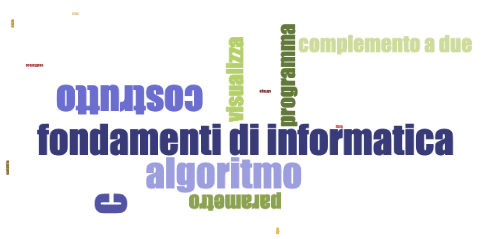
\includegraphics[width=\linewidth]{wcex.png}
  \end{center}%\vspace{-6em}
\end{wrapfigure}

Si vuole realizzare un programma che partendo da un file di testo crei una cosiddetta \textit{Word Cloud} da visualizzarsi mediante una pagina web. Per raggiungere lo scopo, sono dati i seguenti file di testo (disponibili su \texttt{piazza.com}):\begin{itemize}
\item \texttt{stopWords.it.txt} e \texttt{stopWords.txt} che contiene le parole che non vanno considerate in quanto non rilevanti dal punto di vista della semantica (ad esempio congiunzioni, articoli, ...) sia per la lingua italiana che per quella inglese,
\item \texttt{d3.layout.cloud.js}, \texttt{d3.min.js} e \texttt{word-cloud.js} file javascript utilizzati dalla pagina web per realizzare la Word Cloud, e
\item \texttt{wordcloud.htm} pagina html utilizzata per visualizzare la Word Cloud, che include la seguente direttiva: 
\begin{verbatim}
<script type="text/javascript" src="words.js"></script>
\end{verbatim}
Il file \texttt{words.js} \`e ci\`o che il programma deve creare per ottenere il risultato desiderato.
\end{itemize}

Il programma riceve in ingresso un file ASCII contenente il testo da analizzare e crea il file \texttt{words.js} risultato dell'analisi. Il formato di tale file \`e il seguente:
\begin{verbatim}
var tags = [
{"key": "programma", "value" : 26},
{"key": "C", "value" : 27},
{"key": "variabile", "value" : 25},
{"key": "ciclo", "value" : 25},
{"key": "costrutto", "value" : 27},
{"key": "tipo", "value" : 25},
{"key": "sottoprogramma", "value" : 24},
{"key": "parametro", "value" : 26},
{"key": "visualizza", "value" : 26},
{"key": "argc", "value" : 25},
...
{"key": "lista", "value" : 6}
];
\end{verbatim}

A parte la prima e l'ultima riga, ogni elemento specifica un vocabolo quante volte compare nel testo.

Nel realizzare la soluzione, si tengano presente i seguenti aspetti:
\begin{itemize}
\item non mettere nel file finale i vocaboli che compaiono meno di 6 volte;
\item tutti i vocaboli hanno al pi\`u 30 caratteri (simbolo \texttt{LEN}); 
\item i vocaboli contenuti nei file \texttt{stopWords.it.txt} e \texttt{stopWords.txt} sono tutti minuscoli;
\item i vocaboli nel file da analizzare possono avere maiuscole, si tratta di un testo reale;
\item nel file da analizzare ci possono essere segni di interpunzione (virgola, apostrofo, ...) e devono essere opportunamente gestiti;
\item il file da analizzare potrebbe contenere doppi spazi, trovare i vocaboli 
\end{itemize}

A titolo di esempio di ci\`o che dovrebbe realizzare il programma si consideri il testo inziale qui riportato
\vspace{0.5em}
\begin{quotation}
[...] Ai tempi in cui accaddero i fatti che prendiamo a raccontare, quel 
borgo, gi\`a considerabile, era anche un castello, e aveva perci\`o l'onore 
d’alloggiare un comandante, e il vantaggio di possedere una stabile 
guarnigione di soldati spagnoli, che insegnavan la modestia alle fanciulle 
e alle donne del paese, accarezzavan di tempo in tempo le spalle a qualche 
marito, a qualche padre; e, sul finir dell’estate, non mancavan mai di 
spandersi nelle vigne, per diradar l'uve, e alleggerire a' contadini le fatiche 
della vendemmia. Dall'una all'altra di quelle terre [...]
\end{quotation}
\vspace{0.5em}
i vocaboli che il programma dovrebbe considerare, prima di aver ignorato quelli presenti nel file \texttt{stopWords.it.txt} sono:
\vspace{0.5em}
\begin{quotation}
[...] ai tempi in cui accaddero i fatti che prendiamo a raccontare quel borgo gi\`a considerabile era anche un castello e aveva perci\`o onore alloggiare un comandante e il vantaggio di possedere una stabile guarnigione di soldati spagnoli che insegnavan la modestia alle fanciulle e alle donne del paese accarezzavan di tempo in tempo le spalle a qualche marito a qualche padre e sul finir estate non mancavan mai di spandersi nelle vigne per diradar uve e alleggerire contadini le fatiche della vendemmia una altra di quelle terre [...]
\end{quotation}\vspace{0.5em}
utilizzando il file \texttt{stopWords.it.txt}, il programma scarter\`a i vocaboli che compaiono in tale file, arrivando ai seguenti vocaboli (non \`e importante che non ci siano vocaboli ripetuti)
\vspace{0.5em}
\begin{quotation}
tempi fatti prendiamo raccontare borgo considerabile castello onore alloggiare comandante vantaggio possedere stabile guarnigione soldati spagnoli insegnavan modestia fanciulle donne paese accarezzavan tempo tempo spalle marito padre finir estate  mancavan spandersi vigne diradar uve alleggerire contadini fatiche vendemmia terre
\end{quotation}
\vspace{1em}

Si utilizzi il seguente tipo di dato:
\begin{lstlisting}[language=C,numbers=none]
typedef struct wordlist_s {
	char word[LEN+1];
	int times;
	struct wordlist_s * next;
} wordlist_t;
\end{lstlisting}

Si considerino gi\`a a disposizione i seguenti sottoprogrammi (codice disponibile su \texttt{piazza.com}):

\begin{itemize}
\item 
\begin{lstlisting}[language=C]
wordlist_t * increasing(wordlist_t * h, char * w);
\end{lstlisting} 
inserisce un nuovo elemento in ordine alfabetico crescente rispetto al campo \texttt{word} della struttura;
\item
\begin{lstlisting}[language=C]
wordlist_t * deleteptr(wordlist_t * h, wordlist_t * e)
\end{lstlisting} 
elimina un elemento dalla lista;
\item 
\begin{lstlisting}[language=C]
wordlist_t * find(wordlist_t * h , char * w);
\end{lstlisting} 
 trova e restituisce della lista con un certo valore nel campo \texttt{word} della struttura, se esiste, altrimenti restituisce \texttt{NULL}.
\end{itemize}

Si utilizzino i sottoprogrammi delle librerie \texttt{string.h}, \texttt{stdlib.h}, \texttt{ctype.h} e simili quando utili, senza sviluppare ex-novo cose che gi\`a esistono.

\getsol{srccode/wordcloud.c}





\foo{E}{liste ripasso}{09-12-2019}{CB}
%\input{2019-12-09}

\foo{Z}{architettura del calcolatore (hw \& so) -- parte 1}{10-12-2019}{}
%\input{2019-12-10}

\foo{Z}{architettura del calcolatore (hw \& so) -- parte 2}{12-12-2019}{}
%\input{2019-12-11}


\section{Analisi esercizi: partecipazione}
\begin{center}
%    \includegraphics[width=0.9\textwidth]{./flippedExv2h.png}
\end{center}

%
%\foo{E}{array}{12-10-2017}{}
%\input{2017-10-12.array}
%

%
%\foo{E}{array e struct}{17-10-2017}{}
%\input{2017-10-17.arrayestruct}
%
%\foo{L}{algoritmi e array}{18-10-2017}{}
%\input{2017-10-18.lab}
%
%\foo{Z}{stringhe}{19-10-2017}{}
%\input{2017-10-19.stringhe}
%
%\foo{E}{stringhe e strutture}{23-10-2017}{LDT}
%\input{2017-10-23.mixfinoastringhe}
%
%\foo{R}{architettura del calcolatore (hw \& so) -- parte 1}{24-10-2017}{LDT}
%
%\foo{R}{architettura del calcolatore (hw \& so) -- parte 2}{26-10-2017}{LDT}
%
%\foo{Z}{sottoprogrammi}{30-10-2017}{}
%\input{2017-10-30.sottoprogrammi}
%
%\foo{Z}{sottoprogrammi: passaggio parametri e RDA}{31-10-2017}{}
%\input{2017-10-31.sottoprogrammi}
%
%\foo{E}{sottoprogrammi}{02-11-2017}{LDT}
%\input{2017-11-02.sottoprogrammi}
%
%\foo{E}{sottoprogrammi}{06-11-2017}{}
%\input{2017-11-06.sottoprogrammi}
%
%\foo{E}{ricorsione}{07-11-2017}{}
%\input{2017-11-07.ricorsione}
%
%\foo{E}{file}{09-11-2017}{}
%\input{2017-11-09.file}
%
%\foo{E}{file}{16-11-2017}{}
%\input{2017-11-16.file}
%
%\foo{Z}{allocazione dinamica}{16-11-2017}{}
%\input{2017-11-16.allocazionedinamica}
%
%\foo{E}{file, ricorsione e allocazione dinamica}{20-11-2017}{LDT}
%\input{2017-11-20.fileeallocazionedinamica}
%
%\foo{E}{prova d'esame}{21-11-2017}{}
%\input{2017-11-21.provaesame}
%
%\foo{L}{sottoprogrammi}{22-11-2017}{}
%\input{2017-11-22.lab}
%
%\foo{Z}{liste concatenate}{27-11-2017}{}
%\input{2017-11-27.liste}
%
%\foo{Z}{liste concatenate}{28-11-2017}{}
%\input{2017-11-28.liste}
%
%\foo{L}{sottoprogrammi}{29-11-2017}{}
%\input{2017-11-29.lab}
%\sectionbreak
%
%\foo{E}{liste concatenate}{30-11-2017}{}
%\input{2017-11-30.liste}
%
%\foo{E}{liste concatenate}{04-12-2017}{LDT}
%\input{2017-12-04.liste}
%
%\foo{Z}{parametri da riga di comando}{05-12-2017}{}
%\input{2017-12-05.argvargc}
%
%\foo{L}{temi d'esame}{06-12-2017}{}
%\input{2017-12-06.lab}
%\sectionbreak
%
%\foo{E}{temi d'esame}{11-12-2017}{}
%\input{2017-12-11.temidesame}
%
%\foo{E}{temi d'esame}{12-12-2017}{LDT}
%\input{2017-12-12.temidesame}
%
%\foo{L}{temi d'esame}{13-12-2017}{}
%\input{2017-12-13.lab}
%\sectionbreak
%
%\foo{Z}{costrutto \texttt{switch} e linguaggio assembly}{14-12-2017}{}
%\input{2017-12-14.assemblyswitch}
%
%\foo{Z}{temi d'esame}{14-12-2017}{}
%\input{2017-12-14.temidesame}

%\foo{E}{temi d'esame}{18-12-2017}{}
%\input{2017-12-18.temidesame}

\pagebreak

Numero esercizi svolti: \thenumex

Numero esercizi proposti: \thenumexp

\printindex

%\printnomenclature

\end{document}